\documentclass[twoside]{book}

% Packages required by doxygen
\usepackage{fixltx2e}
\usepackage{calc}
\usepackage{doxygen}
\usepackage[export]{adjustbox} % also loads graphicx
\usepackage{graphicx}
\usepackage[utf8]{inputenc}
\usepackage{makeidx}
\usepackage{multicol}
\usepackage{multirow}
\PassOptionsToPackage{warn}{textcomp}
\usepackage{textcomp}
\usepackage[nointegrals]{wasysym}
\usepackage[table]{xcolor}

% Font selection
\usepackage[T1]{fontenc}
\usepackage[scaled=.90]{helvet}
\usepackage{courier}
\usepackage{amssymb}
\usepackage{sectsty}
\renewcommand{\familydefault}{\sfdefault}
\allsectionsfont{%
  \fontseries{bc}\selectfont%
  \color{darkgray}%
}
\renewcommand{\DoxyLabelFont}{%
  \fontseries{bc}\selectfont%
  \color{darkgray}%
}
\newcommand{\+}{\discretionary{\mbox{\scriptsize$\hookleftarrow$}}{}{}}

% Page & text layout
\usepackage{geometry}
\geometry{%
  a4paper,%
  top=2.5cm,%
  bottom=2.5cm,%
  left=2.5cm,%
  right=2.5cm%
}
\tolerance=750
\hfuzz=15pt
\hbadness=750
\setlength{\emergencystretch}{15pt}
\setlength{\parindent}{0cm}
\setlength{\parskip}{3ex plus 2ex minus 2ex}
\makeatletter
\renewcommand{\paragraph}{%
  \@startsection{paragraph}{4}{0ex}{-1.0ex}{1.0ex}{%
    \normalfont\normalsize\bfseries\SS@parafont%
  }%
}
\renewcommand{\subparagraph}{%
  \@startsection{subparagraph}{5}{0ex}{-1.0ex}{1.0ex}{%
    \normalfont\normalsize\bfseries\SS@subparafont%
  }%
}
\makeatother

% Headers & footers
\usepackage{fancyhdr}
\pagestyle{fancyplain}
\fancyhead[LE]{\fancyplain{}{\bfseries\thepage}}
\fancyhead[CE]{\fancyplain{}{}}
\fancyhead[RE]{\fancyplain{}{\bfseries\leftmark}}
\fancyhead[LO]{\fancyplain{}{\bfseries\rightmark}}
\fancyhead[CO]{\fancyplain{}{}}
\fancyhead[RO]{\fancyplain{}{\bfseries\thepage}}
\fancyfoot[LE]{\fancyplain{}{}}
\fancyfoot[CE]{\fancyplain{}{}}
\fancyfoot[RE]{\fancyplain{}{\bfseries\scriptsize Generated by Doxygen }}
\fancyfoot[LO]{\fancyplain{}{\bfseries\scriptsize Generated by Doxygen }}
\fancyfoot[CO]{\fancyplain{}{}}
\fancyfoot[RO]{\fancyplain{}{}}
\renewcommand{\footrulewidth}{0.4pt}
\renewcommand{\chaptermark}[1]{%
  \markboth{#1}{}%
}
\renewcommand{\sectionmark}[1]{%
  \markright{\thesection\ #1}%
}

% Indices & bibliography
\usepackage{natbib}
\usepackage[titles]{tocloft}
\setcounter{tocdepth}{3}
\setcounter{secnumdepth}{5}
\makeindex

% Hyperlinks (required, but should be loaded last)
\usepackage{ifpdf}
\ifpdf
  \usepackage[pdftex,pagebackref=true]{hyperref}
\else
  \usepackage[ps2pdf,pagebackref=true]{hyperref}
\fi
\hypersetup{%
  colorlinks=true,%
  linkcolor=blue,%
  citecolor=blue,%
  unicode%
}

% Custom commands
\newcommand{\clearemptydoublepage}{%
  \newpage{\pagestyle{empty}\cleardoublepage}%
}

\usepackage{caption}
\captionsetup{labelsep=space,justification=centering,font={bf},singlelinecheck=off,skip=4pt,position=top}

%===== C O N T E N T S =====

\begin{document}

% Titlepage & ToC
\hypersetup{pageanchor=false,
             bookmarksnumbered=true,
             pdfencoding=unicode
            }
\pagenumbering{alph}
\begin{titlepage}
\vspace*{7cm}
\begin{center}%
{\Large Philips Hue }\\
\vspace*{1cm}
{\large Generated by Doxygen 1.8.13}\\
\end{center}
\end{titlepage}
\clearemptydoublepage
\pagenumbering{roman}
\tableofcontents
\clearemptydoublepage
\pagenumbering{arabic}
\hypersetup{pageanchor=true}

%--- Begin generated contents ---
\chapter{R\+E\+A\+D\+ME}
\label{md__r_e_a_d_m_e}
\Hypertarget{md__r_e_a_d_m_e}
This is h\+Ue.

A hue dashboard that uses logistic regression to predict when to turn on/off your lights for better home automation.

Completed for C\+S3307 by\+: Gurkiran Tatla Jake Schindler Justine Kim Paul Salvatore Timal Peramune

1) Installation\+: \begin{DoxyVerb}MAC

    Install armadillo using brew:
        brew install armadillo


    Install Wt on Sierra:
        Download wt version 3.3.9 from:
            https://www.webtoolkit.eu/wt/download

        In the wt directory:
            mkdir build
            cd build
            cmake ../

            Note: the next step is very long
            make -j4        

            sudo make DESDIR=/usr/lib install


UBUNTU (VM)

    1) EXPAND THE VM SIZE:

        cd ~/VirtualBox\ VMs/
        cd wt-vm/
        VBoxManage clonehd "wt-vm-disk1.vmdk" "wt-vm_expanded.vdi" --format vdi
        VBoxManage modifyhd "wt-vm_expanded.vdi" --resize 30000

        Then in virtual box go to: Machine > New > Expert Mode
            Name: wt-vm-expanded
            Type: Other
            Version: Other/Unknown (64-bit)
            Memory: 4096 MB

            Under hard disk:
            Use an existing virtual hard disk file, then select wt-vm_expanded.vdi (Normal 29.30GB)

        We will use wt-vm-expanded for the rest of runningYou can then start the vm as normal.

    2) IN CONSOLE OF YOUR COMPUTER, NOT YOUR VM:

        VBoxManage setextradata wt-vm_expanded VBoxInternal2/SharedFoldersEnableSymlinksCreate/wt-vm_expanded 1

    3) INSTALL THE VM GUI (as per instructions posted on owl)

    4) ADD A SHARED FOLDER TO THE VM (as per instructions on owl)

    5) DOWNLOAD JAVA (TO RUN THE EMULATOR ON THE VM)

        sudo apt-get update && sudo apt-get upgrade
        sudo apt-get install software-properties-common
        sudo add-apt-repository ppa:webupd8team/java
        sudo apt-get update
        sudo apt-get install oracle-java8-installer

    6) DOWNLOAD THE HUE EMULATOR AND PLACE INTO THE SHARED FOLDER

        You can download the emulator from:
            https://steveyo.github.io/Hue-Emulator/

        You can run the hue emulator with:
            sudo java -jar HueEmulator-v0.6.jar &

        *** ENSURE THE EMULATOR IS RUNNING ON PORT 8001 ***

    7) DOWNLOAD AND INSTALL OUR DEPENDENCY (ARMADILLO)

        You can download armadillo from:
            http://arma.sourceforge.net/download.html

        Place the unpacked directory onto your ubuntu desktop:
            mv armadillo* ~/Desktop
            cd ~/Desktop/armadillo*

        sudo apt-get install libblas-dev liblapack-dev

        In the armadillo directory:
            cmake .
            make
            sudo make install
\end{DoxyVerb}


2) Compiling \begin{DoxyVerb}chmod 777 build.sh

./build.sh
\end{DoxyVerb}


3) Running \begin{DoxyVerb}chmod 777 run.sh

./run.sh
\end{DoxyVerb}


4) Navigate to \href{http://localhost:8003}{\tt http\+://localhost\+:8003} 
\chapter{Hierarchical Index}
\section{Class Hierarchy}
This inheritance list is sorted roughly, but not completely, alphabetically\+:\begin{DoxyCompactList}
\item \contentsline{section}{args}{\pageref{structargs}}{}
\item \contentsline{section}{Bridge}{\pageref{class_bridge}}{}
\item \contentsline{section}{Persistence}{\pageref{class_persistence}}{}
\item \contentsline{section}{Predict}{\pageref{class_predict}}{}
\item \contentsline{section}{Schedule\+Item}{\pageref{class_schedule_item}}{}
\item \contentsline{section}{State}{\pageref{class_state}}{}
\item \contentsline{section}{User}{\pageref{class_user}}{}
\item W\+Application\begin{DoxyCompactList}
\item \contentsline{section}{Home\+Page}{\pageref{class_home_page}}{}
\end{DoxyCompactList}
\item W\+Push\+Button\begin{DoxyCompactList}
\item \contentsline{section}{Light}{\pageref{class_light}}{}
\item \contentsline{section}{Light\+Group}{\pageref{class_light_group}}{}
\end{DoxyCompactList}
\end{DoxyCompactList}

\chapter{Class Index}
\section{Class List}
Here are the classes, structs, unions and interfaces with brief descriptions\+:\begin{DoxyCompactList}
\item\contentsline{section}{\hyperlink{structargs}{args} \\*Struct to pass args to a new thread }{\pageref{structargs}}{}
\item\contentsline{section}{\hyperlink{class_bridge}{Bridge} }{\pageref{class_bridge}}{}
\item\contentsline{section}{\hyperlink{class_home_page}{Home\+Page} }{\pageref{class_home_page}}{}
\item\contentsline{section}{\hyperlink{class_light}{Light} }{\pageref{class_light}}{}
\item\contentsline{section}{\hyperlink{class_light_group}{Light\+Group} }{\pageref{class_light_group}}{}
\item\contentsline{section}{\hyperlink{class_persistence}{Persistence} \\*A header for the persistence class which contains functions for session-\/to-\/session persistence fo data }{\pageref{class_persistence}}{}
\item\contentsline{section}{\hyperlink{class_predict}{Predict} }{\pageref{class_predict}}{}
\item\contentsline{section}{\hyperlink{class_schedule_item}{Schedule\+Item} }{\pageref{class_schedule_item}}{}
\item\contentsline{section}{\hyperlink{class_state}{State} }{\pageref{class_state}}{}
\item\contentsline{section}{\hyperlink{class_user}{User} }{\pageref{class_user}}{}
\end{DoxyCompactList}

\chapter{Class Documentation}
\hypertarget{structargs}{}\section{args Struct Reference}
\label{structargs}\index{args@{args}}


a struct to pass args to a new thread  


\subsection*{Public Attributes}
\begin{DoxyCompactItemize}
\item 
\mbox{\Hypertarget{structargs_a774aa150d235307ae9383d456c89efac}\label{structargs_a774aa150d235307ae9383d456c89efac}} 
std\+::vector$<$ \hyperlink{class_light}{Light} $\ast$ $>$ {\bfseries lights}
\end{DoxyCompactItemize}


\subsection{Detailed Description}
a struct to pass args to a new thread 

The documentation for this struct was generated from the following file\+:\begin{DoxyCompactItemize}
\item 
Home\+Page.\+cpp\end{DoxyCompactItemize}

\hypertarget{class_bridge}{}\section{Bridge Class Reference}
\label{class_bridge}\index{Bridge@{Bridge}}
\subsection*{Public Member Functions}
\begin{DoxyCompactItemize}
\item 
\mbox{\Hypertarget{class_bridge_ad861a5831395c4960539642a7c8b6d06}\label{class_bridge_ad861a5831395c4960539642a7c8b6d06}} 
{\bfseries Bridge} (std\+::string name, std\+::string location, std\+::string ip, std\+::string port)
\item 
\mbox{\Hypertarget{class_bridge_ae2f074e1112a9f3f65cc780457ba9c53}\label{class_bridge_ae2f074e1112a9f3f65cc780457ba9c53}} 
std\+::string {\bfseries get\+Name} ()
\item 
\mbox{\Hypertarget{class_bridge_a9c807b40340f2469ffad6a8e48bfee73}\label{class_bridge_a9c807b40340f2469ffad6a8e48bfee73}} 
std\+::string {\bfseries get\+Location} ()
\item 
\mbox{\Hypertarget{class_bridge_afe38bfbf62b3da1b3ea8c42f19c34205}\label{class_bridge_afe38bfbf62b3da1b3ea8c42f19c34205}} 
std\+::string {\bfseries get\+IP} ()
\item 
\mbox{\Hypertarget{class_bridge_a46b6c45282e0a62d98d40116b9fb5510}\label{class_bridge_a46b6c45282e0a62d98d40116b9fb5510}} 
std\+::string {\bfseries get\+Port} ()
\item 
\mbox{\Hypertarget{class_bridge_a2eef4d2e75a7d6252199519a6b56146d}\label{class_bridge_a2eef4d2e75a7d6252199519a6b56146d}} 
void {\bfseries set\+Name} (std\+::string)
\item 
\mbox{\Hypertarget{class_bridge_a4208cca29d7abedecb1d57a592a9be30}\label{class_bridge_a4208cca29d7abedecb1d57a592a9be30}} 
void {\bfseries set\+Location} (std\+::string)
\item 
\mbox{\Hypertarget{class_bridge_a3d8c86cedec1777b158bc8edccada592}\label{class_bridge_a3d8c86cedec1777b158bc8edccada592}} 
void {\bfseries set\+IP} (std\+::string)
\item 
\mbox{\Hypertarget{class_bridge_a0552a3f36dd23e8b7e90cf0b5273dadb}\label{class_bridge_a0552a3f36dd23e8b7e90cf0b5273dadb}} 
void {\bfseries set\+Port} (std\+::string)
\end{DoxyCompactItemize}
\subsection*{Private Attributes}
\begin{DoxyCompactItemize}
\item 
\mbox{\Hypertarget{class_bridge_ab637783a4122c0423c513dfc03b314f6}\label{class_bridge_ab637783a4122c0423c513dfc03b314f6}} 
std\+::string {\bfseries name}
\item 
\mbox{\Hypertarget{class_bridge_a04f9fec6433cadffde5fda71a004af96}\label{class_bridge_a04f9fec6433cadffde5fda71a004af96}} 
std\+::string {\bfseries location}
\item 
\mbox{\Hypertarget{class_bridge_a883ece1ead9aa95d8b8bbf5d44049d90}\label{class_bridge_a883ece1ead9aa95d8b8bbf5d44049d90}} 
std\+::string {\bfseries ip}
\item 
\mbox{\Hypertarget{class_bridge_a68fbd2985367915e475d2c16884c9a30}\label{class_bridge_a68fbd2985367915e475d2c16884c9a30}} 
std\+::string {\bfseries port}
\end{DoxyCompactItemize}


The documentation for this class was generated from the following files\+:\begin{DoxyCompactItemize}
\item 
Bridge.\+hpp\item 
Bridge.\+cpp\end{DoxyCompactItemize}

\hypertarget{class_home_page}{}\section{Home\+Page Class Reference}
\label{class_home_page}\index{Home\+Page@{Home\+Page}}
Inheritance diagram for Home\+Page\+:\begin{figure}[H]
\begin{center}
\leavevmode
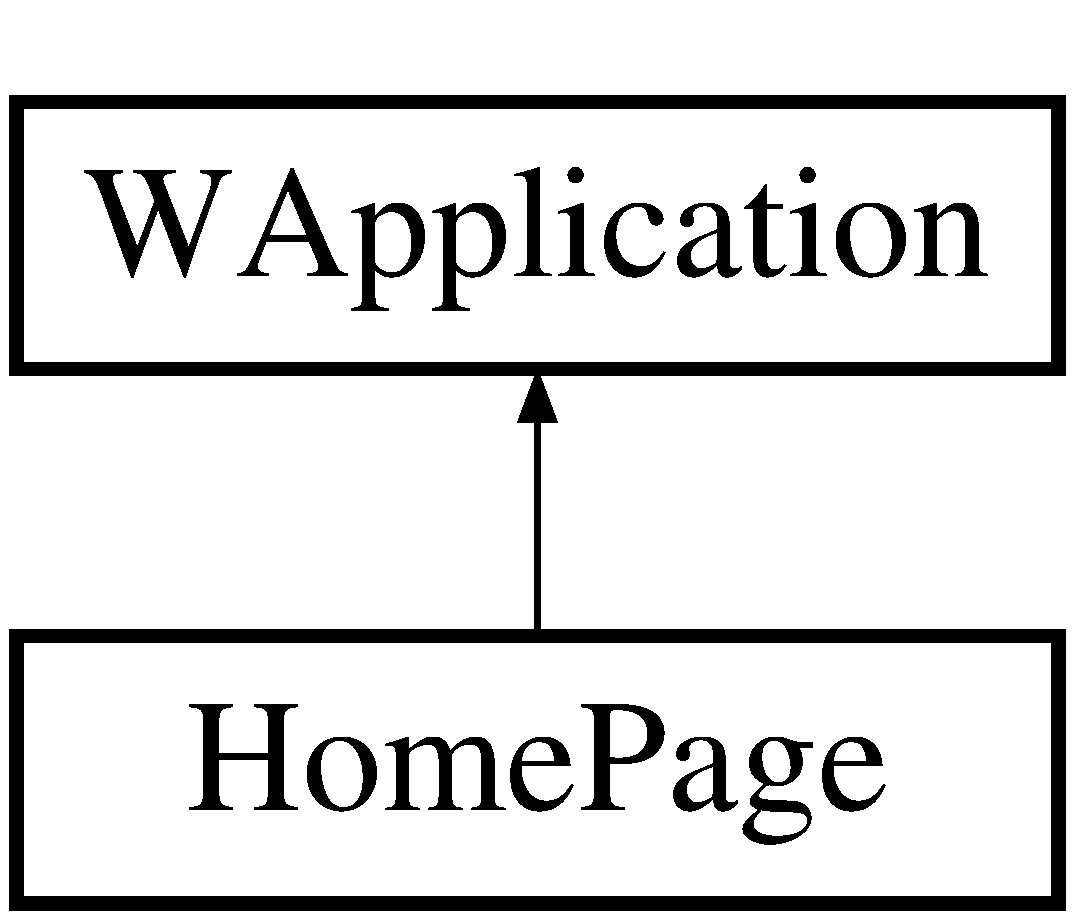
\includegraphics[height=2.000000cm]{class_home_page}
\end{center}
\end{figure}
\subsection*{Public Member Functions}
\begin{DoxyCompactItemize}
\item 
\hyperlink{class_home_page_ae0e5d76697b6796ee71c77555d330eea}{Home\+Page} (const Wt\+::\+W\+Environment \&env)
\begin{DoxyCompactList}\small\item\em the homepage class represents the mission control for the hue lights system \end{DoxyCompactList}\item 
int \hyperlink{class_home_page_a82c2d28ad829b6c8527cec5cefae0104}{get\+Num\+Lights} ()
\begin{DoxyCompactList}\small\item\em gets the number of the lights and return it takes no parameters returns the size of lights (how many there are) \end{DoxyCompactList}\item 
int \hyperlink{class_home_page_a04cc4e1d2ae6d6e1a36c407fa6db8bb4}{get\+Num\+Groups} ()
\begin{DoxyCompactList}\small\item\em returns the number of group \end{DoxyCompactList}\item 
void \hyperlink{class_home_page_adbf50db3ccfa220970c05422495f308a}{change\+Light\+Name} (std\+::string, int)
\begin{DoxyCompactList}\small\item\em takes in the new name String and an integer i ( place in array that light is in) and it changes the light name to that. It had no return value. \end{DoxyCompactList}\item 
void \hyperlink{class_home_page_a5bae10f45d04af24bffdc168e87638a0}{change\+Light\+Hue} (std\+::string, int)
\begin{DoxyCompactList}\small\item\em takes in string cur\+Val and int i (place in array that light is in) and it changes the hue. It has no return value. \end{DoxyCompactList}\item 
void \hyperlink{class_home_page_a748389a4b1b13e026e6d269c4df1f8d5}{change\+Light\+Brightness} (std\+::string, int)
\begin{DoxyCompactList}\small\item\em takes in string bri and int i (place in array that light is in) and it changes the brightness. It has no return value. \end{DoxyCompactList}\item 
void \hyperlink{class_home_page_a515f5cac6f72edd5303f2e1131216640}{change\+Group\+Name} (std\+::string, int)
\begin{DoxyCompactList}\small\item\em changes the name of an existing group \end{DoxyCompactList}\item 
\mbox{\Hypertarget{class_home_page_a46232e6266b10bf35752fc4b2665e668}\label{class_home_page_a46232e6266b10bf35752fc4b2665e668}} 
void {\bfseries change\+Group\+Hue} (std\+::string, int)
\item 
\mbox{\Hypertarget{class_home_page_a2f340e5557757b8040b5ba26b1141442}\label{class_home_page_a2f340e5557757b8040b5ba26b1141442}} 
void {\bfseries change\+Group\+Brightness} (std\+::string, int)
\item 
void \hyperlink{class_home_page_ab85e660ef34d71e7d17872937ee01d7f}{add\+Light\+To\+Group} (std\+::string str)
\begin{DoxyCompactList}\small\item\em adds a light to an existing group \end{DoxyCompactList}\item 
void \hyperlink{class_home_page_ace0313d818ae7561f7707c6fa74f630b}{remove\+Light\+From\+Group} (std\+::string str)
\begin{DoxyCompactList}\small\item\em removes a light to an existing group \end{DoxyCompactList}\item 
void \hyperlink{class_home_page_a0b2d780662f8946abb173e1f3fe136d7}{store\+Light\+Data} ()
\begin{DoxyCompactList}\small\item\em method for creating a thread to store light data \end{DoxyCompactList}\item 
void \hyperlink{class_home_page_ad81aea92b5f0273686d3b25d22ed6d77}{add\+Group} ()
\begin{DoxyCompactList}\small\item\em adds a specified group based on a text input field \end{DoxyCompactList}\item 
void \hyperlink{class_home_page_a019ab5ef1587a197837badfc32725af8}{remove\+Group} ()
\begin{DoxyCompactList}\small\item\em deletes a specified group based on a text input field \end{DoxyCompactList}\item 
\mbox{\Hypertarget{class_home_page_a85bfcacf19ee6acb3186550e5498d119}\label{class_home_page_a85bfcacf19ee6acb3186550e5498d119}} 
\hyperlink{class_bridge}{Bridge} $\ast$ {\bfseries get\+Current\+Bridge} ()
\item 
\hyperlink{class_light}{Light} $\ast$ \hyperlink{class_home_page_ac9c95668c61d02a9ed50675402296d66}{get\+Light\+With\+ID} (std\+::string id)
\begin{DoxyCompactList}\small\item\em get a light with a specific id \end{DoxyCompactList}\end{DoxyCompactItemize}
\subsection*{Private Member Functions}
\begin{DoxyCompactItemize}
\item 
void \hyperlink{class_home_page_a0b1c585653227e946ba3fb0e71a4a7af}{create\+User} ()
\begin{DoxyCompactList}\small\item\em method to create a user, creates a textfile with user\textquotesingle{}s info \end{DoxyCompactList}\item 
void \hyperlink{class_home_page_af34743abfb066e71ef7b1d2f507415eb}{validate\+Login} ()
\begin{DoxyCompactList}\small\item\em method for validating user\textquotesingle{}s login credentials, sets the currentuser to and object of this user if credentials are correct \end{DoxyCompactList}\item 
void \hyperlink{class_home_page_a4dd93ce31ced15fd70992fe6ef67d28b}{update} ()
\begin{DoxyCompactList}\small\item\em method for updating a user\textquotesingle{}s personal and account info \end{DoxyCompactList}\item 
void \hyperlink{class_home_page_aa8de2797f59b77f46f0eaadaec8a63ed}{update\+Password} ()
\begin{DoxyCompactList}\small\item\em method for updating a user\textquotesingle{}s password \end{DoxyCompactList}\item 
\mbox{\Hypertarget{class_home_page_ad75f2a24375568f2c231ce95ced4f1e8}\label{class_home_page_ad75f2a24375568f2c231ce95ced4f1e8}} 
void \hyperlink{class_home_page_ad75f2a24375568f2c231ce95ced4f1e8}{load\+Bridge} ()
\begin{DoxyCompactList}\small\item\em a function that is controlling the UI of the homepage allowing for all Hue light functionality \end{DoxyCompactList}\item 
void \hyperlink{class_home_page_a7ca1f03912ee0763d6fd25e1c4b21eff}{handle\+Http\+Response\+Lights} (boost\+::system\+::error\+\_\+code err, const Wt\+::\+Http\+::\+Message \&response)
\begin{DoxyCompactList}\small\item\em takes an error code err and a message response as parameters and handles the Http Response Lights it. It does not have a return value. \end{DoxyCompactList}\item 
void \hyperlink{class_home_page_a35ecb731b87a0b752be365d42dfa8bf7}{handle\+Http\+Response\+Prediction} (boost\+::system\+::error\+\_\+code err, const Wt\+::\+Http\+::\+Message \&response)
\begin{DoxyCompactList}\small\item\em response from api call to creating a specific scheduled event \end{DoxyCompactList}\item 
void \hyperlink{class_home_page_a7f37c86187bf9bee98eb5f905422eb9c}{handle\+Http\+Response\+Prediction\+Off} (boost\+::system\+::error\+\_\+code err, const Wt\+::\+Http\+::\+Message \&response)
\begin{DoxyCompactList}\small\item\em response from api call to delete a specific scheduled event \end{DoxyCompactList}\item 
void \hyperlink{class_home_page_a84f498dee2335d7f6d11e89105cb82bc}{handle\+Http\+Response\+Get\+Schedule} (boost\+::system\+::error\+\_\+code err, const Wt\+::\+Http\+::\+Message \&response)
\begin{DoxyCompactList}\small\item\em handles the http response after getting all of the current schedule \end{DoxyCompactList}\item 
void \hyperlink{class_home_page_a9fd215402b2cc96281c39454e9c70d69}{handle\+Http\+Response\+Delete\+Schedule} (boost\+::system\+::error\+\_\+code err, const Wt\+::\+Http\+::\+Message \&response)
\begin{DoxyCompactList}\small\item\em handles the http response after deleting a specific schedule \end{DoxyCompactList}\item 
void \hyperlink{class_home_page_a3ece53358d71e7a893cf4284dbcff175}{handle\+Lights\+In\+Groups} (boost\+::system\+::error\+\_\+code err, const Wt\+::\+Http\+::\+Message \&response, int group\+\_\+index)
\begin{DoxyCompactList}\small\item\em adds all lights to their groups \end{DoxyCompactList}\item 
\mbox{\Hypertarget{class_home_page_a0a9851d03cb1adcfe9a28f2546cbd765}\label{class_home_page_a0a9851d03cb1adcfe9a28f2546cbd765}} 
void {\bfseries handle\+Http\+Response\+Groups} (boost\+::system\+::error\+\_\+code err, const Wt\+::\+Http\+::\+Message \&response)
\item 
void \hyperlink{class_home_page_a5a1923f90a2ac6367869f9423e9a3559}{handle\+Http\+Response\+Add\+Bridge} (boost\+::system\+::error\+\_\+code err, const Wt\+::\+Http\+::\+Message \&response)
\begin{DoxyCompactList}\small\item\em method for handling the adding of a bridge \end{DoxyCompactList}\item 
void \hyperlink{class_home_page_a3823da7245637b5b16eec173660661fc}{toggle\+Login} ()
\begin{DoxyCompactList}\small\item\em method for moving between pages \end{DoxyCompactList}\item 
\mbox{\Hypertarget{class_home_page_a25916e36819153779ac8194b2c76c725}\label{class_home_page_a25916e36819153779ac8194b2c76c725}} 
void {\bfseries toggle\+Settings} ()
\item 
\mbox{\Hypertarget{class_home_page_a4121a0ab427705dba5b929d4331f8a9c}\label{class_home_page_a4121a0ab427705dba5b929d4331f8a9c}} 
void {\bfseries toggle\+Home\+Page} ()
\item 
void \hyperlink{class_home_page_a0231c983e866ff4f574d9f26cac7c944}{update\+Bridge\+Text} ()
\begin{DoxyCompactList}\small\item\em method for updating current bridges connected with a user \end{DoxyCompactList}\item 
void \hyperlink{class_home_page_aca01e2e44b307cb44aa0f23ab5d5b25b}{handle\+Create\+Bridge} ()
\begin{DoxyCompactList}\small\item\em method for handling the creation of a bridge \end{DoxyCompactList}\item 
void \hyperlink{class_home_page_a8e33de7e775f85f91d7792eb315b8015}{handle\+Prediction} ()
\begin{DoxyCompactList}\small\item\em creates predicted events using the \hyperlink{class_predict}{Predict} class and logistic regression \end{DoxyCompactList}\item 
void \hyperlink{class_home_page_af6d8f0979312ab9971c4c696992f5096}{handle\+Prediction\+Off} ()
\begin{DoxyCompactList}\small\item\em deletes all events scheduled through predictive mode \end{DoxyCompactList}\item 
void \hyperlink{class_home_page_af449cf14bc9d0196e0cb4a4c352b3919}{handle\+Schedule\+Delete} ()
\begin{DoxyCompactList}\small\item\em a method handling button clicks to delete a particular schedule \end{DoxyCompactList}\item 
void \hyperlink{class_home_page_a1ee49731ce9e0ae4ce8525cd86c800f8}{get\+And\+Display\+Schedule} ()
\begin{DoxyCompactList}\small\item\em makes an api call to get all of the current schedule and prints it to the UI \end{DoxyCompactList}\item 
void \hyperlink{class_home_page_a90f36d7359af291e1becf350c7805768}{handle\+Schedule\+Create\+Light} ()
\begin{DoxyCompactList}\small\item\em calls the handle\+Schedule\+Create for only a light \end{DoxyCompactList}\item 
void \hyperlink{class_home_page_a2e1ef1f628cf82023a688fabfc272bff}{handle\+Schedule\+Create\+Group} ()
\begin{DoxyCompactList}\small\item\em calls the handle\+Schedule\+Create for an entire group \end{DoxyCompactList}\item 
void \hyperlink{class_home_page_ad43b3bb765e485771e9116edbcec0b2b}{handle\+Schedule\+Create} (int group)
\begin{DoxyCompactList}\small\item\em makes an A\+PI to schedule a change dependent on several text fields \end{DoxyCompactList}\item 
void \hyperlink{class_home_page_a8c56067a3cd4dc321572a034d3135ab9}{toggle\+Thread} ()
\begin{DoxyCompactList}\small\item\em turns on/off recording of light states for predictive mode \end{DoxyCompactList}\end{DoxyCompactItemize}
\subsection*{Private Attributes}
\begin{DoxyCompactItemize}
\item 
\mbox{\Hypertarget{class_home_page_ad43f4366a008051d3e1776092b1507fe}\label{class_home_page_ad43f4366a008051d3e1776092b1507fe}} 
std\+::string {\bfseries build\+Current\+Schedule}
\item 
\mbox{\Hypertarget{class_home_page_a8d11f80cbf24a601b1f1b0c553f60f27}\label{class_home_page_a8d11f80cbf24a601b1f1b0c553f60f27}} 
std\+::string {\bfseries delete\+Message}
\item 
\mbox{\Hypertarget{class_home_page_a3542f74573ce071ee708cdd64a09cbb4}\label{class_home_page_a3542f74573ce071ee708cdd64a09cbb4}} 
std\+::vector$<$ \hyperlink{class_light_group}{Light\+Group} $\ast$ $>$ {\bfseries groups}
\item 
\mbox{\Hypertarget{class_home_page_ade2a3d058ec4513037bd3019637b4244}\label{class_home_page_ade2a3d058ec4513037bd3019637b4244}} 
std\+::vector$<$ Wt\+::\+W\+Slider $\ast$ $>$ {\bfseries group\+Hue\+Sliders}
\item 
\mbox{\Hypertarget{class_home_page_ab8b2900ac658e931740f3cb88adbf3f6}\label{class_home_page_ab8b2900ac658e931740f3cb88adbf3f6}} 
std\+::vector$<$ Wt\+::\+W\+Slider $\ast$ $>$ {\bfseries group\+Bri\+Sliders}
\item 
\mbox{\Hypertarget{class_home_page_a3ba52a08e34248ec5c27b09c99d152f1}\label{class_home_page_a3ba52a08e34248ec5c27b09c99d152f1}} 
std\+::vector$<$ Wt\+::\+W\+Line\+Edit $\ast$ $>$ {\bfseries group\+Edits}
\item 
\mbox{\Hypertarget{class_home_page_a83b6a751af68810ab593a87bde1df58e}\label{class_home_page_a83b6a751af68810ab593a87bde1df58e}} 
std\+::vector$<$ \hyperlink{class_light}{Light} $\ast$ $>$ {\bfseries lights}
\item 
\mbox{\Hypertarget{class_home_page_ae86e2fca3964ce3e323ad73c2976882c}\label{class_home_page_ae86e2fca3964ce3e323ad73c2976882c}} 
std\+::string {\bfseries name}
\item 
\mbox{\Hypertarget{class_home_page_a49058000209f6fcf1c3dae010314ab31}\label{class_home_page_a49058000209f6fcf1c3dae010314ab31}} 
std\+::vector$<$ Wt\+::\+W\+Line\+Edit $\ast$ $>$ {\bfseries edits}
\item 
\mbox{\Hypertarget{class_home_page_aff6c1a9092c37bdae536761ee1ab6305}\label{class_home_page_aff6c1a9092c37bdae536761ee1ab6305}} 
std\+::vector$<$ Wt\+::\+W\+Slider $\ast$ $>$ {\bfseries hue\+Sliders}
\item 
\mbox{\Hypertarget{class_home_page_a806a9da2d7a0aecb97e044ae400612c0}\label{class_home_page_a806a9da2d7a0aecb97e044ae400612c0}} 
std\+::vector$<$ Wt\+::\+W\+Slider $\ast$ $>$ {\bfseries brightness\+Sliders}
\item 
\mbox{\Hypertarget{class_home_page_a7d0dd7b2b4bde6726d93d04b88eba8ec}\label{class_home_page_a7d0dd7b2b4bde6726d93d04b88eba8ec}} 
Wt\+::\+W\+Line\+Edit $\ast$ {\bfseries add\+Light\+Edit}
\item 
\mbox{\Hypertarget{class_home_page_a1992b94e871aa02620cd3f3344742978}\label{class_home_page_a1992b94e871aa02620cd3f3344742978}} 
Wt\+::\+W\+Line\+Edit $\ast$ {\bfseries remove\+Light\+Edit}
\item 
\mbox{\Hypertarget{class_home_page_aa923822ce73ff50a6ac80e75ecc34558}\label{class_home_page_aa923822ce73ff50a6ac80e75ecc34558}} 
Wt\+::\+W\+Line\+Edit $\ast$ {\bfseries remove\+Group\+Edit}
\item 
\mbox{\Hypertarget{class_home_page_af0975aebdc40be8d3bb10a4cc0f330b2}\label{class_home_page_af0975aebdc40be8d3bb10a4cc0f330b2}} 
Wt\+::\+W\+Line\+Edit $\ast$ {\bfseries delete\+Schedule\+Id}
\item 
\mbox{\Hypertarget{class_home_page_a863788b73e47f8568bcf34dce9b3a254}\label{class_home_page_a863788b73e47f8568bcf34dce9b3a254}} 
Wt\+::\+W\+Line\+Edit $\ast$ {\bfseries create\+Schedule\+Id}
\item 
\mbox{\Hypertarget{class_home_page_a82efb549e93697236e4b78e7b3e9ee40}\label{class_home_page_a82efb549e93697236e4b78e7b3e9ee40}} 
Wt\+::\+W\+Line\+Edit $\ast$ {\bfseries schedule\+Year}
\item 
\mbox{\Hypertarget{class_home_page_aba574ecf94395d37f557d721e1c76413}\label{class_home_page_aba574ecf94395d37f557d721e1c76413}} 
Wt\+::\+W\+Line\+Edit $\ast$ {\bfseries schedule\+Month}
\item 
\mbox{\Hypertarget{class_home_page_a320665647585bf13dc9cf9a5027f3833}\label{class_home_page_a320665647585bf13dc9cf9a5027f3833}} 
Wt\+::\+W\+Line\+Edit $\ast$ {\bfseries schedule\+Day}
\item 
\mbox{\Hypertarget{class_home_page_a88fc775a2870d436b3ff0c1e08cb7c47}\label{class_home_page_a88fc775a2870d436b3ff0c1e08cb7c47}} 
Wt\+::\+W\+Line\+Edit $\ast$ {\bfseries schedule\+Hour}
\item 
\mbox{\Hypertarget{class_home_page_a7707bae4d9c88faae9180c635890a6a8}\label{class_home_page_a7707bae4d9c88faae9180c635890a6a8}} 
Wt\+::\+W\+Line\+Edit $\ast$ {\bfseries schedule\+Min}
\item 
\mbox{\Hypertarget{class_home_page_a71cbd9da103c3f87e6a6ae9d4fd10205}\label{class_home_page_a71cbd9da103c3f87e6a6ae9d4fd10205}} 
Wt\+::\+W\+Line\+Edit $\ast$ {\bfseries schedule\+On}
\item 
\mbox{\Hypertarget{class_home_page_ac1edd4f5d53f3ed929c1ee4df2948a7d}\label{class_home_page_ac1edd4f5d53f3ed929c1ee4df2948a7d}} 
Wt\+::\+W\+Line\+Edit $\ast$ {\bfseries schedule\+Transition}
\item 
\mbox{\Hypertarget{class_home_page_a48cd37e97a4bda9187f623c4e87be295}\label{class_home_page_a48cd37e97a4bda9187f623c4e87be295}} 
Wt\+::\+W\+Slider $\ast$ {\bfseries schedule\+Hue}
\item 
\mbox{\Hypertarget{class_home_page_a66d374ae4e95029b1b5f8a1fe46722f6}\label{class_home_page_a66d374ae4e95029b1b5f8a1fe46722f6}} 
Wt\+::\+W\+Slider $\ast$ {\bfseries schedule\+Brightness}
\item 
\mbox{\Hypertarget{class_home_page_a7457d428fcd698d60f72c95782b39faf}\label{class_home_page_a7457d428fcd698d60f72c95782b39faf}} 
Wt\+::\+W\+Line\+Edit $\ast$ {\bfseries bridge\+Name}
\item 
\mbox{\Hypertarget{class_home_page_ab04d99877c163415071b9f3a0271513e}\label{class_home_page_ab04d99877c163415071b9f3a0271513e}} 
Wt\+::\+W\+Line\+Edit $\ast$ {\bfseries bridge\+Place}
\item 
\mbox{\Hypertarget{class_home_page_a45fd120ec99938f2bfbce184a9ca7286}\label{class_home_page_a45fd120ec99938f2bfbce184a9ca7286}} 
Wt\+::\+W\+Line\+Edit $\ast$ {\bfseries bridge\+I\+P\+Address}
\item 
\mbox{\Hypertarget{class_home_page_a4969076e3c84a43fd6619b8f979460e8}\label{class_home_page_a4969076e3c84a43fd6619b8f979460e8}} 
Wt\+::\+W\+Line\+Edit $\ast$ {\bfseries bridge\+Port}
\item 
\mbox{\Hypertarget{class_home_page_aaac28b0dd276a70dc3276d41ffa3cab7}\label{class_home_page_aaac28b0dd276a70dc3276d41ffa3cab7}} 
Wt\+::\+W\+Line\+Edit $\ast$ {\bfseries bridge\+Select}
\item 
\mbox{\Hypertarget{class_home_page_a39443293a3c81cd773edb854adff1f06}\label{class_home_page_a39443293a3c81cd773edb854adff1f06}} 
Wt\+::\+W\+Text $\ast$ {\bfseries schedule\+Text}
\item 
\mbox{\Hypertarget{class_home_page_a374f318fc4813cb846eafb26215e87fa}\label{class_home_page_a374f318fc4813cb846eafb26215e87fa}} 
Wt\+::\+W\+Text $\ast$ {\bfseries schedule\+Error\+Text}
\item 
\mbox{\Hypertarget{class_home_page_a5e8e32e17b38b81890ed3d7e1bc54b9f}\label{class_home_page_a5e8e32e17b38b81890ed3d7e1bc54b9f}} 
Wt\+::\+W\+Text $\ast$ {\bfseries prediction\+Text}
\item 
\mbox{\Hypertarget{class_home_page_ac6513658bfdf9e880f413042e1301019}\label{class_home_page_ac6513658bfdf9e880f413042e1301019}} 
Wt\+::\+W\+Push\+Button $\ast$ {\bfseries prediction\+Recording}
\item 
\mbox{\Hypertarget{class_home_page_ad2dd5ad7baa20ba3af98ea202d08cdbd}\label{class_home_page_ad2dd5ad7baa20ba3af98ea202d08cdbd}} 
pthread\+\_\+t {\bfseries worker\+\_\+thread}
\item 
\mbox{\Hypertarget{class_home_page_a8840400b02f213102b90da8dd216532d}\label{class_home_page_a8840400b02f213102b90da8dd216532d}} 
bool {\bfseries thread\+Running}
\item 
\mbox{\Hypertarget{class_home_page_a80e936d1c0377a7422784b8c2ff3ecac}\label{class_home_page_a80e936d1c0377a7422784b8c2ff3ecac}} 
Wt\+::\+W\+Container\+Widget $\ast$ {\bfseries container\+Login}
\item 
\mbox{\Hypertarget{class_home_page_a3b17c835146a6fdc739e0d288bbc3e49}\label{class_home_page_a3b17c835146a6fdc739e0d288bbc3e49}} 
Wt\+::\+W\+Container\+Widget $\ast$ {\bfseries container\+Settings}
\item 
\mbox{\Hypertarget{class_home_page_a4f7587b679365a61fba6deddc7fab620}\label{class_home_page_a4f7587b679365a61fba6deddc7fab620}} 
Wt\+::\+W\+Container\+Widget $\ast$ {\bfseries container\+Home\+Page}
\item 
\mbox{\Hypertarget{class_home_page_a440cbe8e6ee11c653b8fb5e6c5fed0d4}\label{class_home_page_a440cbe8e6ee11c653b8fb5e6c5fed0d4}} 
Wt\+::\+W\+Push\+Button $\ast$ {\bfseries login\+Container\+Btn}
\item 
\mbox{\Hypertarget{class_home_page_a134dd4e29d4eb5b98a3b2c74d02bbc3c}\label{class_home_page_a134dd4e29d4eb5b98a3b2c74d02bbc3c}} 
Wt\+::\+W\+Push\+Button $\ast$ {\bfseries Settings\+Container\+Btn}
\item 
\mbox{\Hypertarget{class_home_page_a733ecbecb3ad83deec5cd6f4257ce0a0}\label{class_home_page_a733ecbecb3ad83deec5cd6f4257ce0a0}} 
Wt\+::\+W\+Push\+Button $\ast$ {\bfseries Home\+Page\+Container\+Btn}
\item 
\mbox{\Hypertarget{class_home_page_a4539d511820e19ecde37af6da7fc1961}\label{class_home_page_a4539d511820e19ecde37af6da7fc1961}} 
Wt\+::\+W\+Line\+Edit $\ast$ {\bfseries email\+Edit\+\_\+}
\item 
\mbox{\Hypertarget{class_home_page_ae8a1d9bcaa453a546d2cd9b1285c7de7}\label{class_home_page_ae8a1d9bcaa453a546d2cd9b1285c7de7}} 
Wt\+::\+W\+Line\+Edit $\ast$ {\bfseries first\+Name\+Edit\+\_\+}
\item 
\mbox{\Hypertarget{class_home_page_abcc21d00e534bf3197eee5d1ab25e8ef}\label{class_home_page_abcc21d00e534bf3197eee5d1ab25e8ef}} 
Wt\+::\+W\+Line\+Edit $\ast$ {\bfseries last\+Name\+Edit\+\_\+}
\item 
\mbox{\Hypertarget{class_home_page_a2af61fdced50fe8fd5c739d6408dee9f}\label{class_home_page_a2af61fdced50fe8fd5c739d6408dee9f}} 
Wt\+::\+W\+Line\+Edit $\ast$ {\bfseries pass\+New\+\_\+}
\item 
\mbox{\Hypertarget{class_home_page_adf3b007a1328192b19ec8d9c6dffe92d}\label{class_home_page_adf3b007a1328192b19ec8d9c6dffe92d}} 
Wt\+::\+W\+Line\+Edit $\ast$ {\bfseries pass\+Old\+\_\+}
\item 
\mbox{\Hypertarget{class_home_page_af249dc7c73669768fdbd68c8f3ce6adc}\label{class_home_page_af249dc7c73669768fdbd68c8f3ce6adc}} 
Wt\+::\+W\+Text $\ast$ {\bfseries change\+Output\+\_\+}
\item 
\mbox{\Hypertarget{class_home_page_ad4a275cc1f6cd29431ed6a51ab1ade8e}\label{class_home_page_ad4a275cc1f6cd29431ed6a51ab1ade8e}} 
Wt\+::\+W\+Text $\ast$ {\bfseries change\+Output\+Pass\+\_\+}
\item 
\mbox{\Hypertarget{class_home_page_a55ecc0d8d1decfadf430b379dea493ea}\label{class_home_page_a55ecc0d8d1decfadf430b379dea493ea}} 
Wt\+::\+W\+Text $\ast$ {\bfseries header\+\_\+}
\item 
\mbox{\Hypertarget{class_home_page_accbb8bdab5a92fcdfb49c4f1b78f7d47}\label{class_home_page_accbb8bdab5a92fcdfb49c4f1b78f7d47}} 
Wt\+::\+W\+Text $\ast$ {\bfseries login\+Text\+\_\+}
\item 
\mbox{\Hypertarget{class_home_page_ae9c814217e8aa38aeb04f4225bba4905}\label{class_home_page_ae9c814217e8aa38aeb04f4225bba4905}} 
Wt\+::\+W\+Text $\ast$ {\bfseries email\+Login\+Text\+\_\+}
\item 
\mbox{\Hypertarget{class_home_page_a62fb2f3ce19da1db8d23b106fbdf00e2}\label{class_home_page_a62fb2f3ce19da1db8d23b106fbdf00e2}} 
Wt\+::\+W\+Text $\ast$ {\bfseries password\+Login\+Text\+\_\+}
\item 
\mbox{\Hypertarget{class_home_page_ade8efdaeb4931e508ff566eeeaf1d579}\label{class_home_page_ade8efdaeb4931e508ff566eeeaf1d579}} 
Wt\+::\+W\+Text $\ast$ {\bfseries create\+Text\+\_\+}
\item 
\mbox{\Hypertarget{class_home_page_adbce88a58a3637315fa91f80e5db9832}\label{class_home_page_adbce88a58a3637315fa91f80e5db9832}} 
Wt\+::\+W\+Text $\ast$ {\bfseries firstname\+\_\+}
\item 
\mbox{\Hypertarget{class_home_page_a06863d54dbc0e8e59568de8e48aa16e4}\label{class_home_page_a06863d54dbc0e8e59568de8e48aa16e4}} 
Wt\+::\+W\+Text $\ast$ {\bfseries lastname\+\_\+}
\item 
\mbox{\Hypertarget{class_home_page_abb09080e7fa8d8e67c3f7b32b36913c6}\label{class_home_page_abb09080e7fa8d8e67c3f7b32b36913c6}} 
Wt\+::\+W\+Text $\ast$ {\bfseries create\+Update\+Text\+\_\+}
\item 
\mbox{\Hypertarget{class_home_page_a4b64b141092c4301da9aefcec1972901}\label{class_home_page_a4b64b141092c4301da9aefcec1972901}} 
Wt\+::\+W\+Text $\ast$ {\bfseries bridge\+Output\+\_\+}
\item 
\mbox{\Hypertarget{class_home_page_a1a83db80bc2079a3c136b921d631d092}\label{class_home_page_a1a83db80bc2079a3c136b921d631d092}} 
Wt\+::\+W\+Line\+Edit $\ast$ {\bfseries email\+Login\+\_\+}
\item 
\mbox{\Hypertarget{class_home_page_aeb262c5638972913967baf59af4ac7fc}\label{class_home_page_aeb262c5638972913967baf59af4ac7fc}} 
Wt\+::\+W\+Line\+Edit $\ast$ {\bfseries password\+Login\+\_\+}
\item 
\mbox{\Hypertarget{class_home_page_a88e1c17d22e0308b1600cbd08a6d4755}\label{class_home_page_a88e1c17d22e0308b1600cbd08a6d4755}} 
Wt\+::\+W\+Line\+Edit $\ast$ {\bfseries email\+Create\+\_\+}
\item 
\mbox{\Hypertarget{class_home_page_a22bd565ef1beace353181e867d21b427}\label{class_home_page_a22bd565ef1beace353181e867d21b427}} 
Wt\+::\+W\+Line\+Edit $\ast$ {\bfseries password\+Create\+\_\+}
\item 
\mbox{\Hypertarget{class_home_page_af28999a99f5ae23b313c0a97cd6f69a2}\label{class_home_page_af28999a99f5ae23b313c0a97cd6f69a2}} 
Wt\+::\+W\+Line\+Edit $\ast$ {\bfseries first\+Create\+\_\+}
\item 
\mbox{\Hypertarget{class_home_page_a219cdf3b4fa7939d9e513d50e413e1d9}\label{class_home_page_a219cdf3b4fa7939d9e513d50e413e1d9}} 
Wt\+::\+W\+Line\+Edit $\ast$ {\bfseries last\+Create\+\_\+}
\item 
\mbox{\Hypertarget{class_home_page_a34949a74a5624d39794e9a36fdc3e3a9}\label{class_home_page_a34949a74a5624d39794e9a36fdc3e3a9}} 
Wt\+::\+W\+Push\+Button $\ast$ {\bfseries login\+Btn}
\item 
\mbox{\Hypertarget{class_home_page_a44aea27c2144dc79e5cd874f1535e3c2}\label{class_home_page_a44aea27c2144dc79e5cd874f1535e3c2}} 
Wt\+::\+W\+Push\+Button $\ast$ {\bfseries create\+Btn}
\item 
\mbox{\Hypertarget{class_home_page_a2906979431ad4c1349096e094388568a}\label{class_home_page_a2906979431ad4c1349096e094388568a}} 
\hyperlink{class_user}{User} $\ast$ {\bfseries user\+Temp}
\item 
\mbox{\Hypertarget{class_home_page_a4f3a9aca2e0316a4a0a7f392677faadb}\label{class_home_page_a4f3a9aca2e0316a4a0a7f392677faadb}} 
\hyperlink{class_user}{User} $\ast$ {\bfseries current\+User}
\item 
\mbox{\Hypertarget{class_home_page_a3bfc1c6ab14d69799d3d39639697726d}\label{class_home_page_a3bfc1c6ab14d69799d3d39639697726d}} 
bool {\bfseries bridge\+Flag}
\item 
\mbox{\Hypertarget{class_home_page_ab045455fa1d609cdafdc4cc3cad23062}\label{class_home_page_ab045455fa1d609cdafdc4cc3cad23062}} 
Wt\+::\+W\+Text $\ast$ {\bfseries bridge\+Status}
\item 
\mbox{\Hypertarget{class_home_page_ae081130ece7aa9b6bba0cc72f793745f}\label{class_home_page_ae081130ece7aa9b6bba0cc72f793745f}} 
std\+::vector$<$ \hyperlink{class_bridge}{Bridge} $\ast$ $>$ {\bfseries bridges}
\item 
\mbox{\Hypertarget{class_home_page_ab5d1ffbc1733044cfb176be7882e24f9}\label{class_home_page_ab5d1ffbc1733044cfb176be7882e24f9}} 
\hyperlink{class_bridge}{Bridge} $\ast$ {\bfseries current\+Bridge}
\end{DoxyCompactItemize}


\subsection{Constructor \& Destructor Documentation}
\mbox{\Hypertarget{class_home_page_ae0e5d76697b6796ee71c77555d330eea}\label{class_home_page_ae0e5d76697b6796ee71c77555d330eea}} 
\index{Home\+Page@{Home\+Page}!Home\+Page@{Home\+Page}}
\index{Home\+Page@{Home\+Page}!Home\+Page@{Home\+Page}}
\subsubsection{\texorpdfstring{Home\+Page()}{HomePage()}}
{\footnotesize\ttfamily Home\+Page\+::\+Home\+Page (\begin{DoxyParamCaption}\item[{const Wt\+::\+W\+Environment \&}]{env }\end{DoxyParamCaption})}



the homepage class represents the mission control for the hue lights system 

\begin{DoxyAuthor}{Author}
Gurkiran Tatla 

Jake Schindler 

Justine Kim 

Paul Salvatore 

Timal Peramune \hyperlink{class_home_page}{Home\+Page} constructor for controlling bridges and user settings
\end{DoxyAuthor}

\begin{DoxyParams}{Parameters}
{\em env} & an envirnmental variable \\
\hline
\end{DoxyParams}
\begin{DoxyReturn}{Returns}
no return value 
\end{DoxyReturn}


\subsection{Member Function Documentation}
\mbox{\Hypertarget{class_home_page_ad81aea92b5f0273686d3b25d22ed6d77}\label{class_home_page_ad81aea92b5f0273686d3b25d22ed6d77}} 
\index{Home\+Page@{Home\+Page}!add\+Group@{add\+Group}}
\index{add\+Group@{add\+Group}!Home\+Page@{Home\+Page}}
\subsubsection{\texorpdfstring{add\+Group()}{addGroup()}}
{\footnotesize\ttfamily void Home\+Page\+::add\+Group (\begin{DoxyParamCaption}{ }\end{DoxyParamCaption})}



adds a specified group based on a text input field 

add\+Group  none \begin{DoxyReturn}{Returns}
none 
\end{DoxyReturn}
\mbox{\Hypertarget{class_home_page_ab85e660ef34d71e7d17872937ee01d7f}\label{class_home_page_ab85e660ef34d71e7d17872937ee01d7f}} 
\index{Home\+Page@{Home\+Page}!add\+Light\+To\+Group@{add\+Light\+To\+Group}}
\index{add\+Light\+To\+Group@{add\+Light\+To\+Group}!Home\+Page@{Home\+Page}}
\subsubsection{\texorpdfstring{add\+Light\+To\+Group()}{addLightToGroup()}}
{\footnotesize\ttfamily void Home\+Page\+::add\+Light\+To\+Group (\begin{DoxyParamCaption}\item[{std\+::string}]{str }\end{DoxyParamCaption})}



adds a light to an existing group 

add\+Light\+To\+Group 
\begin{DoxyParams}{Parameters}
{\em str} & the name of the light to add to the group \\
\hline
\end{DoxyParams}
\begin{DoxyReturn}{Returns}
none 
\end{DoxyReturn}
\mbox{\Hypertarget{class_home_page_a515f5cac6f72edd5303f2e1131216640}\label{class_home_page_a515f5cac6f72edd5303f2e1131216640}} 
\index{Home\+Page@{Home\+Page}!change\+Group\+Name@{change\+Group\+Name}}
\index{change\+Group\+Name@{change\+Group\+Name}!Home\+Page@{Home\+Page}}
\subsubsection{\texorpdfstring{change\+Group\+Name()}{changeGroupName()}}
{\footnotesize\ttfamily void Home\+Page\+::change\+Group\+Name (\begin{DoxyParamCaption}\item[{std\+::string}]{name,  }\item[{int}]{i }\end{DoxyParamCaption})}



changes the name of an existing group 

change\+Group\+Name 
\begin{DoxyParams}{Parameters}
{\em name} & the name we want to change the group to \\
\hline
{\em i} & the index of the group we are renaming \\
\hline
\end{DoxyParams}
\mbox{\Hypertarget{class_home_page_a748389a4b1b13e026e6d269c4df1f8d5}\label{class_home_page_a748389a4b1b13e026e6d269c4df1f8d5}} 
\index{Home\+Page@{Home\+Page}!change\+Light\+Brightness@{change\+Light\+Brightness}}
\index{change\+Light\+Brightness@{change\+Light\+Brightness}!Home\+Page@{Home\+Page}}
\subsubsection{\texorpdfstring{change\+Light\+Brightness()}{changeLightBrightness()}}
{\footnotesize\ttfamily void Home\+Page\+::change\+Light\+Brightness (\begin{DoxyParamCaption}\item[{std\+::string}]{bri,  }\item[{int}]{i }\end{DoxyParamCaption})}



takes in string bri and int i (place in array that light is in) and it changes the brightness. It has no return value. 

change\+Light\+Brightness 
\begin{DoxyParams}{Parameters}
{\em bri} & string representing brightness \\
\hline
{\em i} & int representing place in array \\
\hline
\end{DoxyParams}
\begin{DoxyReturn}{Returns}
nothing 
\end{DoxyReturn}
\mbox{\Hypertarget{class_home_page_a5bae10f45d04af24bffdc168e87638a0}\label{class_home_page_a5bae10f45d04af24bffdc168e87638a0}} 
\index{Home\+Page@{Home\+Page}!change\+Light\+Hue@{change\+Light\+Hue}}
\index{change\+Light\+Hue@{change\+Light\+Hue}!Home\+Page@{Home\+Page}}
\subsubsection{\texorpdfstring{change\+Light\+Hue()}{changeLightHue()}}
{\footnotesize\ttfamily void Home\+Page\+::change\+Light\+Hue (\begin{DoxyParamCaption}\item[{std\+::string}]{cur\+Val,  }\item[{int}]{i }\end{DoxyParamCaption})}



takes in string cur\+Val and int i (place in array that light is in) and it changes the hue. It has no return value. 

change\+Light\+Hue 
\begin{DoxyParams}{Parameters}
{\em cur\+Val} & string representing hue \\
\hline
{\em i} & int representing place in array \\
\hline
\end{DoxyParams}
\begin{DoxyReturn}{Returns}
nothing 
\end{DoxyReturn}
\mbox{\Hypertarget{class_home_page_adbf50db3ccfa220970c05422495f308a}\label{class_home_page_adbf50db3ccfa220970c05422495f308a}} 
\index{Home\+Page@{Home\+Page}!change\+Light\+Name@{change\+Light\+Name}}
\index{change\+Light\+Name@{change\+Light\+Name}!Home\+Page@{Home\+Page}}
\subsubsection{\texorpdfstring{change\+Light\+Name()}{changeLightName()}}
{\footnotesize\ttfamily void Home\+Page\+::change\+Light\+Name (\begin{DoxyParamCaption}\item[{std\+::string}]{name,  }\item[{int}]{i }\end{DoxyParamCaption})}



takes in the new name String and an integer i ( place in array that light is in) and it changes the light name to that. It had no return value. 

change\+Light\+Name 
\begin{DoxyParams}{Parameters}
{\em name} & string for the new light name \\
\hline
{\em i} & int representing place in array \\
\hline
\end{DoxyParams}
\begin{DoxyReturn}{Returns}
nothing 
\end{DoxyReturn}
\mbox{\Hypertarget{class_home_page_a0b1c585653227e946ba3fb0e71a4a7af}\label{class_home_page_a0b1c585653227e946ba3fb0e71a4a7af}} 
\index{Home\+Page@{Home\+Page}!create\+User@{create\+User}}
\index{create\+User@{create\+User}!Home\+Page@{Home\+Page}}
\subsubsection{\texorpdfstring{create\+User()}{createUser()}}
{\footnotesize\ttfamily void Home\+Page\+::create\+User (\begin{DoxyParamCaption}{ }\end{DoxyParamCaption})\hspace{0.3cm}{\ttfamily [private]}}



method to create a user, creates a textfile with user\textquotesingle{}s info 

\hyperlink{class_home_page_a0231c983e866ff4f574d9f26cac7c944}{Home\+Page\+::update\+Bridge\+Text} 
\begin{DoxyParams}{Parameters}
{\em args} & none \\
\hline
\end{DoxyParams}
\begin{DoxyReturn}{Returns}
void$\ast$\+: returns void 
\end{DoxyReturn}
\mbox{\Hypertarget{class_home_page_a1ee49731ce9e0ae4ce8525cd86c800f8}\label{class_home_page_a1ee49731ce9e0ae4ce8525cd86c800f8}} 
\index{Home\+Page@{Home\+Page}!get\+And\+Display\+Schedule@{get\+And\+Display\+Schedule}}
\index{get\+And\+Display\+Schedule@{get\+And\+Display\+Schedule}!Home\+Page@{Home\+Page}}
\subsubsection{\texorpdfstring{get\+And\+Display\+Schedule()}{getAndDisplaySchedule()}}
{\footnotesize\ttfamily void Home\+Page\+::get\+And\+Display\+Schedule (\begin{DoxyParamCaption}{ }\end{DoxyParamCaption})\hspace{0.3cm}{\ttfamily [private]}}



makes an api call to get all of the current schedule and prints it to the UI 

get\+And\+Display\+Schedule 
\begin{DoxyParams}{Parameters}
{\em none} & \\
\hline
\end{DoxyParams}
\begin{DoxyReturn}{Returns}
none 
\end{DoxyReturn}
\mbox{\Hypertarget{class_home_page_ac9c95668c61d02a9ed50675402296d66}\label{class_home_page_ac9c95668c61d02a9ed50675402296d66}} 
\index{Home\+Page@{Home\+Page}!get\+Light\+With\+ID@{get\+Light\+With\+ID}}
\index{get\+Light\+With\+ID@{get\+Light\+With\+ID}!Home\+Page@{Home\+Page}}
\subsubsection{\texorpdfstring{get\+Light\+With\+I\+D()}{getLightWithID()}}
{\footnotesize\ttfamily \hyperlink{class_light}{Light} $\ast$ Home\+Page\+::get\+Light\+With\+ID (\begin{DoxyParamCaption}\item[{std\+::string}]{id }\end{DoxyParamCaption})}



get a light with a specific id 

get\+Light\+With\+ID 
\begin{DoxyParams}{Parameters}
{\em id} & a string representing the id of a light to get \\
\hline
\end{DoxyParams}
\begin{DoxyReturn}{Returns}
null if the light does not exist, otherwise returns the light pointer object 
\end{DoxyReturn}
\mbox{\Hypertarget{class_home_page_a04cc4e1d2ae6d6e1a36c407fa6db8bb4}\label{class_home_page_a04cc4e1d2ae6d6e1a36c407fa6db8bb4}} 
\index{Home\+Page@{Home\+Page}!get\+Num\+Groups@{get\+Num\+Groups}}
\index{get\+Num\+Groups@{get\+Num\+Groups}!Home\+Page@{Home\+Page}}
\subsubsection{\texorpdfstring{get\+Num\+Groups()}{getNumGroups()}}
{\footnotesize\ttfamily int Home\+Page\+::get\+Num\+Groups (\begin{DoxyParamCaption}{ }\end{DoxyParamCaption})}



returns the number of group 

get\+Num\+Groups 
\begin{DoxyParams}{Parameters}
{\em none} & \\
\hline
\end{DoxyParams}
\begin{DoxyReturn}{Returns}
an int representing the number of groups 
\end{DoxyReturn}
\mbox{\Hypertarget{class_home_page_a82c2d28ad829b6c8527cec5cefae0104}\label{class_home_page_a82c2d28ad829b6c8527cec5cefae0104}} 
\index{Home\+Page@{Home\+Page}!get\+Num\+Lights@{get\+Num\+Lights}}
\index{get\+Num\+Lights@{get\+Num\+Lights}!Home\+Page@{Home\+Page}}
\subsubsection{\texorpdfstring{get\+Num\+Lights()}{getNumLights()}}
{\footnotesize\ttfamily int Home\+Page\+::get\+Num\+Lights (\begin{DoxyParamCaption}{ }\end{DoxyParamCaption})}



gets the number of the lights and return it takes no parameters returns the size of lights (how many there are) 

get\+Num\+Lights 
\begin{DoxyParams}{Parameters}
{\em none} & \\
\hline
\end{DoxyParams}
\begin{DoxyReturn}{Returns}
an int representing the number of lights 
\end{DoxyReturn}
\mbox{\Hypertarget{class_home_page_aca01e2e44b307cb44aa0f23ab5d5b25b}\label{class_home_page_aca01e2e44b307cb44aa0f23ab5d5b25b}} 
\index{Home\+Page@{Home\+Page}!handle\+Create\+Bridge@{handle\+Create\+Bridge}}
\index{handle\+Create\+Bridge@{handle\+Create\+Bridge}!Home\+Page@{Home\+Page}}
\subsubsection{\texorpdfstring{handle\+Create\+Bridge()}{handleCreateBridge()}}
{\footnotesize\ttfamily void Home\+Page\+::handle\+Create\+Bridge (\begin{DoxyParamCaption}{ }\end{DoxyParamCaption})\hspace{0.3cm}{\ttfamily [private]}}



method for handling the creation of a bridge 

\hyperlink{class_home_page_a5a1923f90a2ac6367869f9423e9a3559}{Home\+Page\+::handle\+Http\+Response\+Add\+Bridge} 
\begin{DoxyParams}{Parameters}
{\em args} & none \\
\hline
\end{DoxyParams}
\begin{DoxyReturn}{Returns}
void$\ast$\+: returns void 
\end{DoxyReturn}
\mbox{\Hypertarget{class_home_page_a5a1923f90a2ac6367869f9423e9a3559}\label{class_home_page_a5a1923f90a2ac6367869f9423e9a3559}} 
\index{Home\+Page@{Home\+Page}!handle\+Http\+Response\+Add\+Bridge@{handle\+Http\+Response\+Add\+Bridge}}
\index{handle\+Http\+Response\+Add\+Bridge@{handle\+Http\+Response\+Add\+Bridge}!Home\+Page@{Home\+Page}}
\subsubsection{\texorpdfstring{handle\+Http\+Response\+Add\+Bridge()}{handleHttpResponseAddBridge()}}
{\footnotesize\ttfamily void Home\+Page\+::handle\+Http\+Response\+Add\+Bridge (\begin{DoxyParamCaption}\item[{boost\+::system\+::error\+\_\+code}]{err,  }\item[{const Wt\+::\+Http\+::\+Message \&}]{response }\end{DoxyParamCaption})\hspace{0.3cm}{\ttfamily [private]}}



method for handling the adding of a bridge 

\hyperlink{class_home_page_a5a1923f90a2ac6367869f9423e9a3559}{Home\+Page\+::handle\+Http\+Response\+Add\+Bridge} 
\begin{DoxyParams}{Parameters}
{\em args} & boost\+::system\+::error\+\_\+code err, const Wt\+::\+Http\+::\+Message \&response \\
\hline
\end{DoxyParams}
\begin{DoxyReturn}{Returns}
void$\ast$\+: returns void 
\end{DoxyReturn}
\mbox{\Hypertarget{class_home_page_a9fd215402b2cc96281c39454e9c70d69}\label{class_home_page_a9fd215402b2cc96281c39454e9c70d69}} 
\index{Home\+Page@{Home\+Page}!handle\+Http\+Response\+Delete\+Schedule@{handle\+Http\+Response\+Delete\+Schedule}}
\index{handle\+Http\+Response\+Delete\+Schedule@{handle\+Http\+Response\+Delete\+Schedule}!Home\+Page@{Home\+Page}}
\subsubsection{\texorpdfstring{handle\+Http\+Response\+Delete\+Schedule()}{handleHttpResponseDeleteSchedule()}}
{\footnotesize\ttfamily void Home\+Page\+::handle\+Http\+Response\+Delete\+Schedule (\begin{DoxyParamCaption}\item[{boost\+::system\+::error\+\_\+code}]{err,  }\item[{const Wt\+::\+Http\+::\+Message \&}]{response }\end{DoxyParamCaption})\hspace{0.3cm}{\ttfamily [private]}}



handles the http response after deleting a specific schedule 

handle\+Http\+Response\+Delete\+Schedule 
\begin{DoxyParams}{Parameters}
{\em err} & a boost err variable \\
\hline
{\em response} & a Wt http message response variable \\
\hline
\end{DoxyParams}
\begin{DoxyReturn}{Returns}
none 
\end{DoxyReturn}
\mbox{\Hypertarget{class_home_page_a84f498dee2335d7f6d11e89105cb82bc}\label{class_home_page_a84f498dee2335d7f6d11e89105cb82bc}} 
\index{Home\+Page@{Home\+Page}!handle\+Http\+Response\+Get\+Schedule@{handle\+Http\+Response\+Get\+Schedule}}
\index{handle\+Http\+Response\+Get\+Schedule@{handle\+Http\+Response\+Get\+Schedule}!Home\+Page@{Home\+Page}}
\subsubsection{\texorpdfstring{handle\+Http\+Response\+Get\+Schedule()}{handleHttpResponseGetSchedule()}}
{\footnotesize\ttfamily void Home\+Page\+::handle\+Http\+Response\+Get\+Schedule (\begin{DoxyParamCaption}\item[{boost\+::system\+::error\+\_\+code}]{err,  }\item[{const Wt\+::\+Http\+::\+Message \&}]{response }\end{DoxyParamCaption})\hspace{0.3cm}{\ttfamily [private]}}



handles the http response after getting all of the current schedule 

handle\+Http\+Response\+Get\+Schedule 
\begin{DoxyParams}{Parameters}
{\em err} & a boost err variable \\
\hline
{\em response} & a Wt http message response variable \\
\hline
\end{DoxyParams}
\begin{DoxyReturn}{Returns}
none 
\end{DoxyReturn}
\mbox{\Hypertarget{class_home_page_a7ca1f03912ee0763d6fd25e1c4b21eff}\label{class_home_page_a7ca1f03912ee0763d6fd25e1c4b21eff}} 
\index{Home\+Page@{Home\+Page}!handle\+Http\+Response\+Lights@{handle\+Http\+Response\+Lights}}
\index{handle\+Http\+Response\+Lights@{handle\+Http\+Response\+Lights}!Home\+Page@{Home\+Page}}
\subsubsection{\texorpdfstring{handle\+Http\+Response\+Lights()}{handleHttpResponseLights()}}
{\footnotesize\ttfamily void Home\+Page\+::handle\+Http\+Response\+Lights (\begin{DoxyParamCaption}\item[{boost\+::system\+::error\+\_\+code}]{err,  }\item[{const Wt\+::\+Http\+::\+Message \&}]{response }\end{DoxyParamCaption})\hspace{0.3cm}{\ttfamily [private]}}



takes an error code err and a message response as parameters and handles the Http Response Lights it. It does not have a return value. 

handle\+Http\+Response\+Lights 
\begin{DoxyParams}{Parameters}
{\em err} & error code \\
\hline
{\em response} & message response \\
\hline
\end{DoxyParams}
\begin{DoxyReturn}{Returns}
nothing 
\end{DoxyReturn}
\mbox{\Hypertarget{class_home_page_a35ecb731b87a0b752be365d42dfa8bf7}\label{class_home_page_a35ecb731b87a0b752be365d42dfa8bf7}} 
\index{Home\+Page@{Home\+Page}!handle\+Http\+Response\+Prediction@{handle\+Http\+Response\+Prediction}}
\index{handle\+Http\+Response\+Prediction@{handle\+Http\+Response\+Prediction}!Home\+Page@{Home\+Page}}
\subsubsection{\texorpdfstring{handle\+Http\+Response\+Prediction()}{handleHttpResponsePrediction()}}
{\footnotesize\ttfamily void Home\+Page\+::handle\+Http\+Response\+Prediction (\begin{DoxyParamCaption}\item[{boost\+::system\+::error\+\_\+code}]{err,  }\item[{const Wt\+::\+Http\+::\+Message \&}]{response }\end{DoxyParamCaption})\hspace{0.3cm}{\ttfamily [private]}}



response from api call to creating a specific scheduled event 

handle\+Http\+Response\+Prediction 
\begin{DoxyParams}{Parameters}
{\em err} & a boost err variable \\
\hline
{\em response} & a Wt http message response variable \\
\hline
\end{DoxyParams}
\begin{DoxyReturn}{Returns}
none 
\end{DoxyReturn}
\mbox{\Hypertarget{class_home_page_a7f37c86187bf9bee98eb5f905422eb9c}\label{class_home_page_a7f37c86187bf9bee98eb5f905422eb9c}} 
\index{Home\+Page@{Home\+Page}!handle\+Http\+Response\+Prediction\+Off@{handle\+Http\+Response\+Prediction\+Off}}
\index{handle\+Http\+Response\+Prediction\+Off@{handle\+Http\+Response\+Prediction\+Off}!Home\+Page@{Home\+Page}}
\subsubsection{\texorpdfstring{handle\+Http\+Response\+Prediction\+Off()}{handleHttpResponsePredictionOff()}}
{\footnotesize\ttfamily void Home\+Page\+::handle\+Http\+Response\+Prediction\+Off (\begin{DoxyParamCaption}\item[{boost\+::system\+::error\+\_\+code}]{err,  }\item[{const Wt\+::\+Http\+::\+Message \&}]{response }\end{DoxyParamCaption})\hspace{0.3cm}{\ttfamily [private]}}



response from api call to delete a specific scheduled event 

handle\+Http\+Response\+Prediction\+Off 
\begin{DoxyParams}{Parameters}
{\em err} & a boost err variable \\
\hline
{\em response} & a Wt http message response variable \\
\hline
\end{DoxyParams}
\begin{DoxyReturn}{Returns}
none 
\end{DoxyReturn}
\mbox{\Hypertarget{class_home_page_a3ece53358d71e7a893cf4284dbcff175}\label{class_home_page_a3ece53358d71e7a893cf4284dbcff175}} 
\index{Home\+Page@{Home\+Page}!handle\+Lights\+In\+Groups@{handle\+Lights\+In\+Groups}}
\index{handle\+Lights\+In\+Groups@{handle\+Lights\+In\+Groups}!Home\+Page@{Home\+Page}}
\subsubsection{\texorpdfstring{handle\+Lights\+In\+Groups()}{handleLightsInGroups()}}
{\footnotesize\ttfamily void Home\+Page\+::handle\+Lights\+In\+Groups (\begin{DoxyParamCaption}\item[{boost\+::system\+::error\+\_\+code}]{err,  }\item[{const Wt\+::\+Http\+::\+Message \&}]{response,  }\item[{int}]{group\+\_\+index }\end{DoxyParamCaption})\hspace{0.3cm}{\ttfamily [private]}}



adds all lights to their groups 

handle\+Lights\+In\+Groups 
\begin{DoxyParams}{Parameters}
{\em err} & a boost err variable \\
\hline
{\em response} & a Wt http message response variable \\
\hline
{\em group\+\_\+index} & the integer index of the group we are adding to \\
\hline
\end{DoxyParams}
\begin{DoxyReturn}{Returns}
none 
\end{DoxyReturn}
\mbox{\Hypertarget{class_home_page_a8e33de7e775f85f91d7792eb315b8015}\label{class_home_page_a8e33de7e775f85f91d7792eb315b8015}} 
\index{Home\+Page@{Home\+Page}!handle\+Prediction@{handle\+Prediction}}
\index{handle\+Prediction@{handle\+Prediction}!Home\+Page@{Home\+Page}}
\subsubsection{\texorpdfstring{handle\+Prediction()}{handlePrediction()}}
{\footnotesize\ttfamily void Home\+Page\+::handle\+Prediction (\begin{DoxyParamCaption}{ }\end{DoxyParamCaption})\hspace{0.3cm}{\ttfamily [private]}}



creates predicted events using the \hyperlink{class_predict}{Predict} class and logistic regression 

handle\+Prediction 
\begin{DoxyParams}{Parameters}
{\em none} & \\
\hline
\end{DoxyParams}
\begin{DoxyReturn}{Returns}
none 
\end{DoxyReturn}
\mbox{\Hypertarget{class_home_page_af6d8f0979312ab9971c4c696992f5096}\label{class_home_page_af6d8f0979312ab9971c4c696992f5096}} 
\index{Home\+Page@{Home\+Page}!handle\+Prediction\+Off@{handle\+Prediction\+Off}}
\index{handle\+Prediction\+Off@{handle\+Prediction\+Off}!Home\+Page@{Home\+Page}}
\subsubsection{\texorpdfstring{handle\+Prediction\+Off()}{handlePredictionOff()}}
{\footnotesize\ttfamily void Home\+Page\+::handle\+Prediction\+Off (\begin{DoxyParamCaption}{ }\end{DoxyParamCaption})\hspace{0.3cm}{\ttfamily [private]}}



deletes all events scheduled through predictive mode 

handle\+Prediction\+Off 
\begin{DoxyParams}{Parameters}
{\em none} & \\
\hline
\end{DoxyParams}
\begin{DoxyReturn}{Returns}
none 
\end{DoxyReturn}
\mbox{\Hypertarget{class_home_page_ad43b3bb765e485771e9116edbcec0b2b}\label{class_home_page_ad43b3bb765e485771e9116edbcec0b2b}} 
\index{Home\+Page@{Home\+Page}!handle\+Schedule\+Create@{handle\+Schedule\+Create}}
\index{handle\+Schedule\+Create@{handle\+Schedule\+Create}!Home\+Page@{Home\+Page}}
\subsubsection{\texorpdfstring{handle\+Schedule\+Create()}{handleScheduleCreate()}}
{\footnotesize\ttfamily void Home\+Page\+::handle\+Schedule\+Create (\begin{DoxyParamCaption}\item[{int}]{group }\end{DoxyParamCaption})\hspace{0.3cm}{\ttfamily [private]}}



makes an A\+PI to schedule a change dependent on several text fields 

handle\+Schedule\+Create 
\begin{DoxyParams}{Parameters}
{\em group} & an int (0 or 1) representing whether to schedule a light, or group, respectively \\
\hline
\end{DoxyParams}
\begin{DoxyReturn}{Returns}
none 
\end{DoxyReturn}
\mbox{\Hypertarget{class_home_page_a2e1ef1f628cf82023a688fabfc272bff}\label{class_home_page_a2e1ef1f628cf82023a688fabfc272bff}} 
\index{Home\+Page@{Home\+Page}!handle\+Schedule\+Create\+Group@{handle\+Schedule\+Create\+Group}}
\index{handle\+Schedule\+Create\+Group@{handle\+Schedule\+Create\+Group}!Home\+Page@{Home\+Page}}
\subsubsection{\texorpdfstring{handle\+Schedule\+Create\+Group()}{handleScheduleCreateGroup()}}
{\footnotesize\ttfamily void Home\+Page\+::handle\+Schedule\+Create\+Group (\begin{DoxyParamCaption}{ }\end{DoxyParamCaption})\hspace{0.3cm}{\ttfamily [private]}}



calls the handle\+Schedule\+Create for an entire group 

handle\+Schedule\+Create\+Light 
\begin{DoxyParams}{Parameters}
{\em none} & \\
\hline
\end{DoxyParams}
\begin{DoxyReturn}{Returns}
none 
\end{DoxyReturn}
\mbox{\Hypertarget{class_home_page_a90f36d7359af291e1becf350c7805768}\label{class_home_page_a90f36d7359af291e1becf350c7805768}} 
\index{Home\+Page@{Home\+Page}!handle\+Schedule\+Create\+Light@{handle\+Schedule\+Create\+Light}}
\index{handle\+Schedule\+Create\+Light@{handle\+Schedule\+Create\+Light}!Home\+Page@{Home\+Page}}
\subsubsection{\texorpdfstring{handle\+Schedule\+Create\+Light()}{handleScheduleCreateLight()}}
{\footnotesize\ttfamily void Home\+Page\+::handle\+Schedule\+Create\+Light (\begin{DoxyParamCaption}{ }\end{DoxyParamCaption})\hspace{0.3cm}{\ttfamily [private]}}



calls the handle\+Schedule\+Create for only a light 

handle\+Schedule\+Create\+Light 
\begin{DoxyParams}{Parameters}
{\em none} & \\
\hline
\end{DoxyParams}
\begin{DoxyReturn}{Returns}
none 
\end{DoxyReturn}
\mbox{\Hypertarget{class_home_page_af449cf14bc9d0196e0cb4a4c352b3919}\label{class_home_page_af449cf14bc9d0196e0cb4a4c352b3919}} 
\index{Home\+Page@{Home\+Page}!handle\+Schedule\+Delete@{handle\+Schedule\+Delete}}
\index{handle\+Schedule\+Delete@{handle\+Schedule\+Delete}!Home\+Page@{Home\+Page}}
\subsubsection{\texorpdfstring{handle\+Schedule\+Delete()}{handleScheduleDelete()}}
{\footnotesize\ttfamily void Home\+Page\+::handle\+Schedule\+Delete (\begin{DoxyParamCaption}{ }\end{DoxyParamCaption})\hspace{0.3cm}{\ttfamily [private]}}



a method handling button clicks to delete a particular schedule 

handle\+Schedule\+Delete 
\begin{DoxyParams}{Parameters}
{\em none} & \\
\hline
\end{DoxyParams}
\begin{DoxyReturn}{Returns}
none 
\end{DoxyReturn}
\mbox{\Hypertarget{class_home_page_a019ab5ef1587a197837badfc32725af8}\label{class_home_page_a019ab5ef1587a197837badfc32725af8}} 
\index{Home\+Page@{Home\+Page}!remove\+Group@{remove\+Group}}
\index{remove\+Group@{remove\+Group}!Home\+Page@{Home\+Page}}
\subsubsection{\texorpdfstring{remove\+Group()}{removeGroup()}}
{\footnotesize\ttfamily void Home\+Page\+::remove\+Group (\begin{DoxyParamCaption}{ }\end{DoxyParamCaption})}



deletes a specified group based on a text input field 

remove\+Group  none \begin{DoxyReturn}{Returns}
none 
\end{DoxyReturn}
\mbox{\Hypertarget{class_home_page_ace0313d818ae7561f7707c6fa74f630b}\label{class_home_page_ace0313d818ae7561f7707c6fa74f630b}} 
\index{Home\+Page@{Home\+Page}!remove\+Light\+From\+Group@{remove\+Light\+From\+Group}}
\index{remove\+Light\+From\+Group@{remove\+Light\+From\+Group}!Home\+Page@{Home\+Page}}
\subsubsection{\texorpdfstring{remove\+Light\+From\+Group()}{removeLightFromGroup()}}
{\footnotesize\ttfamily void Home\+Page\+::remove\+Light\+From\+Group (\begin{DoxyParamCaption}\item[{std\+::string}]{str }\end{DoxyParamCaption})}



removes a light to an existing group 

remove\+Light\+From\+Group 
\begin{DoxyParams}{Parameters}
{\em str} & the name of the light to removes from the group \\
\hline
\end{DoxyParams}
\begin{DoxyReturn}{Returns}
none 
\end{DoxyReturn}
\mbox{\Hypertarget{class_home_page_a0b2d780662f8946abb173e1f3fe136d7}\label{class_home_page_a0b2d780662f8946abb173e1f3fe136d7}} 
\index{Home\+Page@{Home\+Page}!store\+Light\+Data@{store\+Light\+Data}}
\index{store\+Light\+Data@{store\+Light\+Data}!Home\+Page@{Home\+Page}}
\subsubsection{\texorpdfstring{store\+Light\+Data()}{storeLightData()}}
{\footnotesize\ttfamily void Home\+Page\+::store\+Light\+Data (\begin{DoxyParamCaption}{ }\end{DoxyParamCaption})}



method for creating a thread to store light data 

store\+Light\+Data 
\begin{DoxyParams}{Parameters}
{\em none} & \\
\hline
\end{DoxyParams}
\begin{DoxyReturn}{Returns}
none 
\end{DoxyReturn}
\mbox{\Hypertarget{class_home_page_a3823da7245637b5b16eec173660661fc}\label{class_home_page_a3823da7245637b5b16eec173660661fc}} 
\index{Home\+Page@{Home\+Page}!toggle\+Login@{toggle\+Login}}
\index{toggle\+Login@{toggle\+Login}!Home\+Page@{Home\+Page}}
\subsubsection{\texorpdfstring{toggle\+Login()}{toggleLogin()}}
{\footnotesize\ttfamily void Home\+Page\+::toggle\+Login (\begin{DoxyParamCaption}{ }\end{DoxyParamCaption})\hspace{0.3cm}{\ttfamily [private]}}



method for moving between pages 

\hyperlink{class_home_page_a3823da7245637b5b16eec173660661fc}{Home\+Page\+::toggle\+Login}, Home\+Page\+::toggle\+Settings, Home\+Page\+::toggle\+Home\+Page 
\begin{DoxyParams}{Parameters}
{\em args} & none \\
\hline
\end{DoxyParams}
\begin{DoxyReturn}{Returns}
void$\ast$\+: returns void 
\end{DoxyReturn}
\mbox{\Hypertarget{class_home_page_a8c56067a3cd4dc321572a034d3135ab9}\label{class_home_page_a8c56067a3cd4dc321572a034d3135ab9}} 
\index{Home\+Page@{Home\+Page}!toggle\+Thread@{toggle\+Thread}}
\index{toggle\+Thread@{toggle\+Thread}!Home\+Page@{Home\+Page}}
\subsubsection{\texorpdfstring{toggle\+Thread()}{toggleThread()}}
{\footnotesize\ttfamily void Home\+Page\+::toggle\+Thread (\begin{DoxyParamCaption}{ }\end{DoxyParamCaption})\hspace{0.3cm}{\ttfamily [private]}}



turns on/off recording of light states for predictive mode 

toggle\+Thread 
\begin{DoxyParams}{Parameters}
{\em none} & \\
\hline
\end{DoxyParams}
\begin{DoxyReturn}{Returns}
none 
\end{DoxyReturn}
\mbox{\Hypertarget{class_home_page_a4dd93ce31ced15fd70992fe6ef67d28b}\label{class_home_page_a4dd93ce31ced15fd70992fe6ef67d28b}} 
\index{Home\+Page@{Home\+Page}!update@{update}}
\index{update@{update}!Home\+Page@{Home\+Page}}
\subsubsection{\texorpdfstring{update()}{update()}}
{\footnotesize\ttfamily void Home\+Page\+::update (\begin{DoxyParamCaption}{ }\end{DoxyParamCaption})\hspace{0.3cm}{\ttfamily [private]}}



method for updating a user\textquotesingle{}s personal and account info 

\hyperlink{class_home_page_a4dd93ce31ced15fd70992fe6ef67d28b}{Home\+Page\+::update} 
\begin{DoxyParams}{Parameters}
{\em args} & none \\
\hline
\end{DoxyParams}
\begin{DoxyReturn}{Returns}
void$\ast$\+: returns void 
\end{DoxyReturn}
\mbox{\Hypertarget{class_home_page_a0231c983e866ff4f574d9f26cac7c944}\label{class_home_page_a0231c983e866ff4f574d9f26cac7c944}} 
\index{Home\+Page@{Home\+Page}!update\+Bridge\+Text@{update\+Bridge\+Text}}
\index{update\+Bridge\+Text@{update\+Bridge\+Text}!Home\+Page@{Home\+Page}}
\subsubsection{\texorpdfstring{update\+Bridge\+Text()}{updateBridgeText()}}
{\footnotesize\ttfamily void Home\+Page\+::update\+Bridge\+Text (\begin{DoxyParamCaption}{ }\end{DoxyParamCaption})\hspace{0.3cm}{\ttfamily [private]}}



method for updating current bridges connected with a user 

\hyperlink{class_home_page_a0231c983e866ff4f574d9f26cac7c944}{Home\+Page\+::update\+Bridge\+Text} 
\begin{DoxyParams}{Parameters}
{\em args} & none \\
\hline
\end{DoxyParams}
\begin{DoxyReturn}{Returns}
void$\ast$\+: returns void 
\end{DoxyReturn}
\mbox{\Hypertarget{class_home_page_aa8de2797f59b77f46f0eaadaec8a63ed}\label{class_home_page_aa8de2797f59b77f46f0eaadaec8a63ed}} 
\index{Home\+Page@{Home\+Page}!update\+Password@{update\+Password}}
\index{update\+Password@{update\+Password}!Home\+Page@{Home\+Page}}
\subsubsection{\texorpdfstring{update\+Password()}{updatePassword()}}
{\footnotesize\ttfamily void Home\+Page\+::update\+Password (\begin{DoxyParamCaption}{ }\end{DoxyParamCaption})\hspace{0.3cm}{\ttfamily [private]}}



method for updating a user\textquotesingle{}s password 

\hyperlink{class_home_page_aa8de2797f59b77f46f0eaadaec8a63ed}{Home\+Page\+::update\+Password} 
\begin{DoxyParams}{Parameters}
{\em args} & none \\
\hline
\end{DoxyParams}
\begin{DoxyReturn}{Returns}
void$\ast$\+: returns void 
\end{DoxyReturn}
\mbox{\Hypertarget{class_home_page_af34743abfb066e71ef7b1d2f507415eb}\label{class_home_page_af34743abfb066e71ef7b1d2f507415eb}} 
\index{Home\+Page@{Home\+Page}!validate\+Login@{validate\+Login}}
\index{validate\+Login@{validate\+Login}!Home\+Page@{Home\+Page}}
\subsubsection{\texorpdfstring{validate\+Login()}{validateLogin()}}
{\footnotesize\ttfamily void Home\+Page\+::validate\+Login (\begin{DoxyParamCaption}{ }\end{DoxyParamCaption})\hspace{0.3cm}{\ttfamily [private]}}



method for validating user\textquotesingle{}s login credentials, sets the currentuser to and object of this user if credentials are correct 

\hyperlink{class_home_page_af34743abfb066e71ef7b1d2f507415eb}{Home\+Page\+::validate\+Login} 
\begin{DoxyParams}{Parameters}
{\em args} & none \\
\hline
\end{DoxyParams}
\begin{DoxyReturn}{Returns}
void$\ast$\+: returns void 
\end{DoxyReturn}


The documentation for this class was generated from the following files\+:\begin{DoxyCompactItemize}
\item 
Home\+Page.\+hpp\item 
Home\+Page.\+cpp\end{DoxyCompactItemize}

\hypertarget{class_light}{}\section{Light Class Reference}
\label{class_light}\index{Light@{Light}}
Inheritance diagram for Light\+:\begin{figure}[H]
\begin{center}
\leavevmode
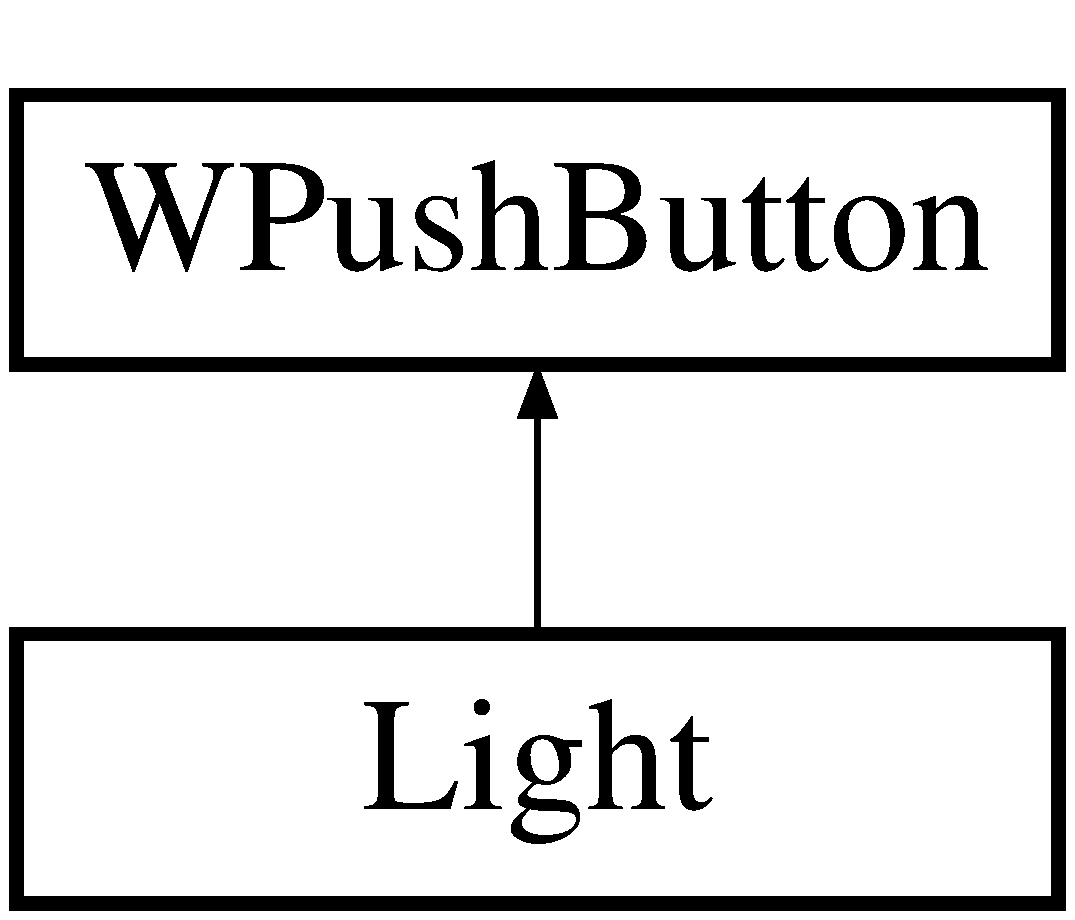
\includegraphics[height=2.000000cm]{class_light}
\end{center}
\end{figure}
\subsection*{Public Member Functions}
\begin{DoxyCompactItemize}
\item 
\hyperlink{class_light_a51f6d94b66ec884ce479ae481de8247b}{Light} (std\+::string id, std\+::string name, \hyperlink{class_home_page}{Home\+Page} $\ast$page)
\begin{DoxyCompactList}\small\item\em The light class which represents a Hue light with it\textquotesingle{}s associated state. \end{DoxyCompactList}\item 
\hyperlink{class_light_a190b96270bfc664d1e209a5055330f40}{Light} (std\+::string id, std\+::string name, \hyperlink{class_state}{State} $\ast$state, \hyperlink{class_home_page}{Home\+Page} $\ast$page)
\begin{DoxyCompactList}\small\item\em Constructor; Initialization function to create a \hyperlink{class_light}{Light}. \end{DoxyCompactList}\item 
\mbox{\Hypertarget{class_light_ace49d0a563a4e9711e03b144465e6e55}\label{class_light_ace49d0a563a4e9711e03b144465e6e55}} 
{\bfseries Light} (std\+::string id, std\+::string name, \hyperlink{class_home_page}{Home\+Page} $\ast$page, \hyperlink{class_state}{State} $\ast$state)
\item 
\hyperlink{class_light_ad0e59fad13bb6cfadc25b2c477e9ddc7}{$\sim$\+Light} ()
\begin{DoxyCompactList}\small\item\em Deconstructor. \end{DoxyCompactList}\item 
\hyperlink{class_state}{State} $\ast$ \hyperlink{class_light_a287da1d58d038e10899c38f8464cbc22}{get\+State} ()
\begin{DoxyCompactList}\small\item\em Returns the \hyperlink{class_state}{State} of the \hyperlink{class_light}{Light}; must always be called with every light object created. \end{DoxyCompactList}\item 
void \hyperlink{class_light_aaa50f42697fdae36ec4b021098fac974}{set\+Name} (std\+::string name, std\+::string ip, std\+::string port)
\begin{DoxyCompactList}\small\item\em sets the name of the light \end{DoxyCompactList}\item 
std\+::string \hyperlink{class_light_a248c379885ea63ee7d71f7e19b0dab80}{get\+Name} ()
\begin{DoxyCompactList}\small\item\em Returns the name of the \hyperlink{class_light}{Light}. \end{DoxyCompactList}\item 
std\+::string \hyperlink{class_light_a7a41305231132e8bae6a899b703fd39a}{get\+ID} ()
\begin{DoxyCompactList}\small\item\em Returns the ID of the \hyperlink{class_light}{Light}. \end{DoxyCompactList}\item 
void \hyperlink{class_light_ab22e6d81d0ccb2f844d404e2e038f9a2}{turn\+O\+Nor\+O\+FF} ()
\begin{DoxyCompactList}\small\item\em Turns the light on or off. \end{DoxyCompactList}\item 
void \hyperlink{class_light_addc99af8c89bfd9c0ebd8908bd290ba7}{set\+Hue} (long long hue)
\begin{DoxyCompactList}\small\item\em Sets the hue of the \hyperlink{class_light}{Light}. \end{DoxyCompactList}\item 
void \hyperlink{class_light_a95d42b02b50ea8f060be6efa0481ba3c}{set\+Brightness} (int brightness)
\begin{DoxyCompactList}\small\item\em Sets the brightness of the \hyperlink{class_light}{Light}. \end{DoxyCompactList}\end{DoxyCompactItemize}
\subsection*{Private Attributes}
\begin{DoxyCompactItemize}
\item 
\mbox{\Hypertarget{class_light_a3aede2c7bf6a2e7596e3b93735470b6d}\label{class_light_a3aede2c7bf6a2e7596e3b93735470b6d}} 
std\+::string {\bfseries id}
\item 
\mbox{\Hypertarget{class_light_aed2e518d1e739c50c31ae77a865f51ed}\label{class_light_aed2e518d1e739c50c31ae77a865f51ed}} 
std\+::string {\bfseries name}
\item 
\mbox{\Hypertarget{class_light_a6f17ea47d17e0536c67cd13e230953ad}\label{class_light_a6f17ea47d17e0536c67cd13e230953ad}} 
\hyperlink{class_state}{State} $\ast$ {\bfseries state}
\item 
\mbox{\Hypertarget{class_light_a0cc3c685f7ee10e6c2925d8ba660ce61}\label{class_light_a0cc3c685f7ee10e6c2925d8ba660ce61}} 
\hyperlink{class_home_page}{Home\+Page} $\ast$ {\bfseries page}
\end{DoxyCompactItemize}


\subsection{Constructor \& Destructor Documentation}
\mbox{\Hypertarget{class_light_a51f6d94b66ec884ce479ae481de8247b}\label{class_light_a51f6d94b66ec884ce479ae481de8247b}} 
\index{Light@{Light}!Light@{Light}}
\index{Light@{Light}!Light@{Light}}
\subsubsection{\texorpdfstring{Light()}{Light()}\hspace{0.1cm}{\footnotesize\ttfamily [1/2]}}
{\footnotesize\ttfamily Light\+::\+Light (\begin{DoxyParamCaption}\item[{std\+::string}]{id,  }\item[{std\+::string}]{name,  }\item[{\hyperlink{class_home_page}{Home\+Page} $\ast$}]{page }\end{DoxyParamCaption})}



The light class which represents a Hue light with it\textquotesingle{}s associated state. 

\begin{DoxyAuthor}{Author}
Gurkiran Tatla 

Jake Schindler 

Justine Kim 

Paul Salvatore 

Timal Peramune \hyperlink{class_light_a51f6d94b66ec884ce479ae481de8247b}{Light\+::\+Light(std\+::string id, std\+::string name, Home\+Page $\ast$page)} Constructor; Initialization function to create a \hyperlink{class_light}{Light}
\end{DoxyAuthor}

\begin{DoxyParams}{Parameters}
{\em id} & an ID number for the \hyperlink{class_light}{Light} \\
\hline
{\em name} & a name for the \hyperlink{class_light}{Light} \\
\hline
{\em \hyperlink{class_home_page}{Home\+Page}} & $\ast$page\+: link to homepage \\
\hline
\end{DoxyParams}
\begin{DoxyReturn}{Returns}
N/A 
\end{DoxyReturn}
\mbox{\Hypertarget{class_light_a190b96270bfc664d1e209a5055330f40}\label{class_light_a190b96270bfc664d1e209a5055330f40}} 
\index{Light@{Light}!Light@{Light}}
\index{Light@{Light}!Light@{Light}}
\subsubsection{\texorpdfstring{Light()}{Light()}\hspace{0.1cm}{\footnotesize\ttfamily [2/2]}}
{\footnotesize\ttfamily Light\+::\+Light (\begin{DoxyParamCaption}\item[{std\+::string}]{id,  }\item[{std\+::string}]{name,  }\item[{\hyperlink{class_state}{State} $\ast$}]{state,  }\item[{\hyperlink{class_home_page}{Home\+Page} $\ast$}]{page }\end{DoxyParamCaption})}



Constructor; Initialization function to create a \hyperlink{class_light}{Light}. 

Light\+::\+Light(std\+::string id, std\+::string name, Home\+Page $\ast$page, State $\ast$state) 
\begin{DoxyParams}{Parameters}
{\em id} & an ID number for the light \\
\hline
{\em name} & a name for the light \\
\hline
{\em page} & homepage \\
\hline
{\em \hyperlink{class_state}{State}} & light state \\
\hline
\end{DoxyParams}
\begin{DoxyReturn}{Returns}
N/A 
\end{DoxyReturn}
\mbox{\Hypertarget{class_light_ad0e59fad13bb6cfadc25b2c477e9ddc7}\label{class_light_ad0e59fad13bb6cfadc25b2c477e9ddc7}} 
\index{Light@{Light}!````~Light@{$\sim$\+Light}}
\index{````~Light@{$\sim$\+Light}!Light@{Light}}
\subsubsection{\texorpdfstring{$\sim$\+Light()}{~Light()}}
{\footnotesize\ttfamily Light\+::$\sim$\+Light (\begin{DoxyParamCaption}{ }\end{DoxyParamCaption})}



Deconstructor. 

\hyperlink{class_light_ad0e59fad13bb6cfadc25b2c477e9ddc7}{Light\+::$\sim$\+Light()} 
\begin{DoxyParams}{Parameters}
{\em N/A} & \\
\hline
\end{DoxyParams}
\begin{DoxyReturn}{Returns}
N/A 
\end{DoxyReturn}


\subsection{Member Function Documentation}
\mbox{\Hypertarget{class_light_a7a41305231132e8bae6a899b703fd39a}\label{class_light_a7a41305231132e8bae6a899b703fd39a}} 
\index{Light@{Light}!get\+ID@{get\+ID}}
\index{get\+ID@{get\+ID}!Light@{Light}}
\subsubsection{\texorpdfstring{get\+I\+D()}{getID()}}
{\footnotesize\ttfamily std\+::string Light\+::get\+ID (\begin{DoxyParamCaption}{ }\end{DoxyParamCaption})}



Returns the ID of the \hyperlink{class_light}{Light}. 

\hyperlink{class_light_a7a41305231132e8bae6a899b703fd39a}{Light\+::get\+I\+D()} 
\begin{DoxyParams}{Parameters}
{\em N/A} & \\
\hline
\end{DoxyParams}
\begin{DoxyReturn}{Returns}
std\+::string\+: ID of the light 
\end{DoxyReturn}
\mbox{\Hypertarget{class_light_a248c379885ea63ee7d71f7e19b0dab80}\label{class_light_a248c379885ea63ee7d71f7e19b0dab80}} 
\index{Light@{Light}!get\+Name@{get\+Name}}
\index{get\+Name@{get\+Name}!Light@{Light}}
\subsubsection{\texorpdfstring{get\+Name()}{getName()}}
{\footnotesize\ttfamily std\+::string Light\+::get\+Name (\begin{DoxyParamCaption}{ }\end{DoxyParamCaption})}



Returns the name of the \hyperlink{class_light}{Light}. 

\hyperlink{class_light_a248c379885ea63ee7d71f7e19b0dab80}{Light\+::get\+Name()} 
\begin{DoxyParams}{Parameters}
{\em N/A} & \\
\hline
\end{DoxyParams}
\begin{DoxyReturn}{Returns}
std\+::string\+: name of the light 
\end{DoxyReturn}
\mbox{\Hypertarget{class_light_a287da1d58d038e10899c38f8464cbc22}\label{class_light_a287da1d58d038e10899c38f8464cbc22}} 
\index{Light@{Light}!get\+State@{get\+State}}
\index{get\+State@{get\+State}!Light@{Light}}
\subsubsection{\texorpdfstring{get\+State()}{getState()}}
{\footnotesize\ttfamily \hyperlink{class_state}{State} $\ast$ Light\+::get\+State (\begin{DoxyParamCaption}{ }\end{DoxyParamCaption})}



Returns the \hyperlink{class_state}{State} of the \hyperlink{class_light}{Light}; must always be called with every light object created. 

\hyperlink{class_light_a287da1d58d038e10899c38f8464cbc22}{Light\+::get\+State()} 
\begin{DoxyParams}{Parameters}
{\em N/A} & \\
\hline
\end{DoxyParams}
\begin{DoxyReturn}{Returns}
\hyperlink{class_state}{State}\+: state of the light 
\end{DoxyReturn}
\mbox{\Hypertarget{class_light_a95d42b02b50ea8f060be6efa0481ba3c}\label{class_light_a95d42b02b50ea8f060be6efa0481ba3c}} 
\index{Light@{Light}!set\+Brightness@{set\+Brightness}}
\index{set\+Brightness@{set\+Brightness}!Light@{Light}}
\subsubsection{\texorpdfstring{set\+Brightness()}{setBrightness()}}
{\footnotesize\ttfamily void Light\+::set\+Brightness (\begin{DoxyParamCaption}\item[{int}]{brightness }\end{DoxyParamCaption})}



Sets the brightness of the \hyperlink{class_light}{Light}. 

\hyperlink{class_light_a95d42b02b50ea8f060be6efa0481ba3c}{Light\+::set\+Brightness(int brightness)} 
\begin{DoxyParams}{Parameters}
{\em brightness} & an int to represent the brightness of the light \\
\hline
\end{DoxyParams}
\begin{DoxyReturn}{Returns}
N/A 
\end{DoxyReturn}
\mbox{\Hypertarget{class_light_addc99af8c89bfd9c0ebd8908bd290ba7}\label{class_light_addc99af8c89bfd9c0ebd8908bd290ba7}} 
\index{Light@{Light}!set\+Hue@{set\+Hue}}
\index{set\+Hue@{set\+Hue}!Light@{Light}}
\subsubsection{\texorpdfstring{set\+Hue()}{setHue()}}
{\footnotesize\ttfamily void Light\+::set\+Hue (\begin{DoxyParamCaption}\item[{long long}]{hue }\end{DoxyParamCaption})}



Sets the hue of the \hyperlink{class_light}{Light}. 

\hyperlink{class_light_addc99af8c89bfd9c0ebd8908bd290ba7}{Light\+::set\+Hue(long long hue)} 
\begin{DoxyParams}{Parameters}
{\em hue} & a long to represent the hue of the light \\
\hline
\end{DoxyParams}
\begin{DoxyReturn}{Returns}
N/A 
\end{DoxyReturn}
\mbox{\Hypertarget{class_light_aaa50f42697fdae36ec4b021098fac974}\label{class_light_aaa50f42697fdae36ec4b021098fac974}} 
\index{Light@{Light}!set\+Name@{set\+Name}}
\index{set\+Name@{set\+Name}!Light@{Light}}
\subsubsection{\texorpdfstring{set\+Name()}{setName()}}
{\footnotesize\ttfamily void Light\+::set\+Name (\begin{DoxyParamCaption}\item[{std\+::string}]{name,  }\item[{std\+::string}]{ip,  }\item[{std\+::string}]{port }\end{DoxyParamCaption})}



sets the name of the light 

Light\+::set\+Name(std\+::string name) 
\begin{DoxyParams}{Parameters}
{\em name} & name of the light \\
\hline
\end{DoxyParams}
\begin{DoxyReturn}{Returns}
N/A 
\end{DoxyReturn}
\mbox{\Hypertarget{class_light_ab22e6d81d0ccb2f844d404e2e038f9a2}\label{class_light_ab22e6d81d0ccb2f844d404e2e038f9a2}} 
\index{Light@{Light}!turn\+O\+Nor\+O\+FF@{turn\+O\+Nor\+O\+FF}}
\index{turn\+O\+Nor\+O\+FF@{turn\+O\+Nor\+O\+FF}!Light@{Light}}
\subsubsection{\texorpdfstring{turn\+O\+Nor\+O\+F\+F()}{turnONorOFF()}}
{\footnotesize\ttfamily void Light\+::turn\+O\+Nor\+O\+FF (\begin{DoxyParamCaption}{ }\end{DoxyParamCaption})}



Turns the light on or off. 

\hyperlink{class_light_ab22e6d81d0ccb2f844d404e2e038f9a2}{Light\+::turn\+O\+Nor\+O\+F\+F()} 
\begin{DoxyParams}{Parameters}
{\em N/A} & \\
\hline
\end{DoxyParams}
\begin{DoxyReturn}{Returns}
N/A 
\end{DoxyReturn}


The documentation for this class was generated from the following files\+:\begin{DoxyCompactItemize}
\item 
Light.\+hpp\item 
Light.\+cpp\end{DoxyCompactItemize}

\hypertarget{class_light_group}{}\section{Light\+Group Class Reference}
\label{class_light_group}\index{Light\+Group@{Light\+Group}}
Inheritance diagram for Light\+Group\+:\begin{figure}[H]
\begin{center}
\leavevmode
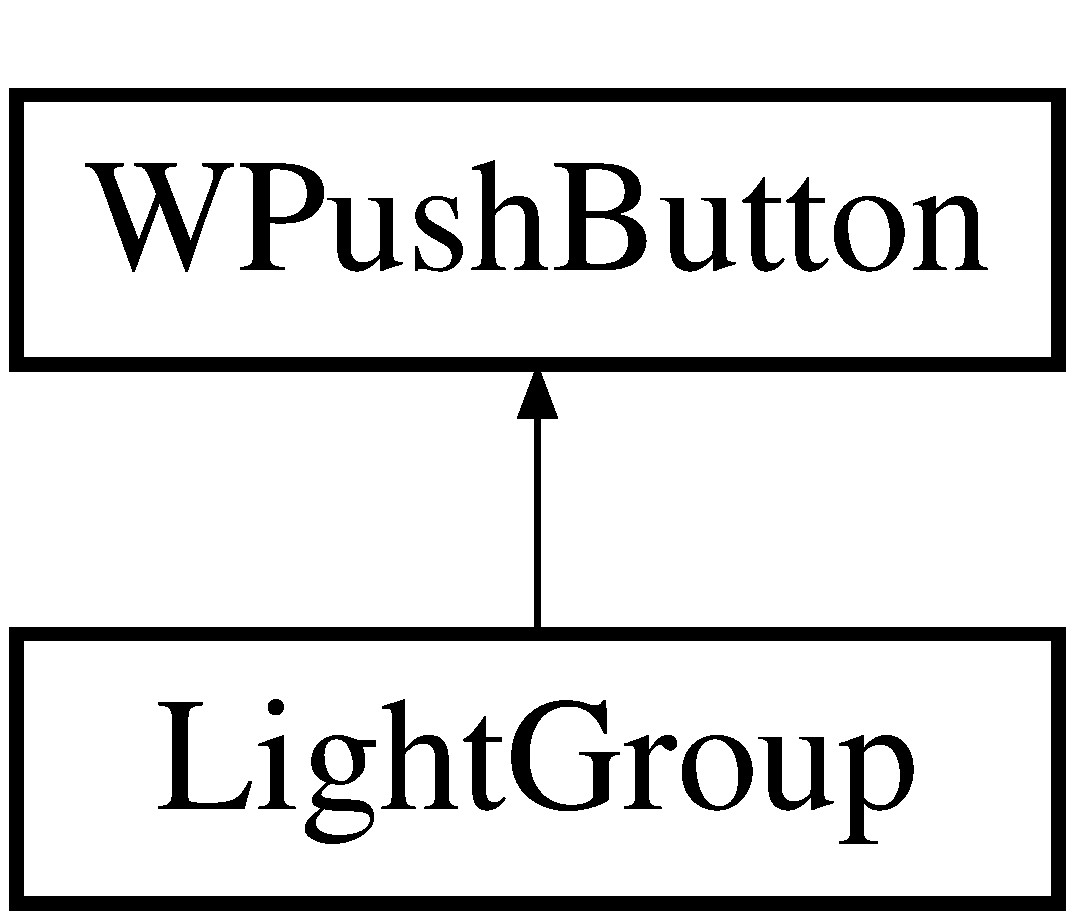
\includegraphics[height=2.000000cm]{class_light_group}
\end{center}
\end{figure}
\subsection*{Public Member Functions}
\begin{DoxyCompactItemize}
\item 
\hyperlink{class_light_group_a640052573b06ee856b04158f83835210}{Light\+Group} (std\+::string id, std\+::string name, \hyperlink{class_home_page}{Home\+Page} $\ast$page, std\+::string ip, std\+::string port)
\begin{DoxyCompactList}\small\item\em The lightgroup class which represents the groups of lights on the hue bridge. \end{DoxyCompactList}\item 
void \hyperlink{class_light_group_a31d089214736e7c6d9896a4977a9e956}{set\+Name} (std\+::string name, std\+::string ip, std\+::string port)
\item 
void \hyperlink{class_light_group_a1586f3bce7da99ab50e6e35f9598effd}{add\+Light} (\hyperlink{class_light}{Light} $\ast$light)
\begin{DoxyCompactList}\small\item\em add a light to the light group \end{DoxyCompactList}\item 
void \hyperlink{class_light_group_a4c401d9a379641cfad1a5aa643a91e25}{remove\+Light} (\hyperlink{class_light}{Light} $\ast$light)
\begin{DoxyCompactList}\small\item\em remove a light from the light group \end{DoxyCompactList}\item 
std\+::string \hyperlink{class_light_group_a8bcdd2d8d6acfbdeac93c0708bddebf5}{get\+Name} ()
\begin{DoxyCompactList}\small\item\em get the name of the lightgroup \end{DoxyCompactList}\item 
std\+::string \hyperlink{class_light_group_af2a28bb84204d5cd64420ea213e86d8d}{get\+ID} ()
\begin{DoxyCompactList}\small\item\em get the id of the lightgroup \end{DoxyCompactList}\item 
std\+::string $\ast$ \hyperlink{class_light_group_a9e5a81ac9940935dbc87a3a33ebe7fc4}{get\+All\+Light\+Names} ()
\begin{DoxyCompactList}\small\item\em gets the names of every light in the group \end{DoxyCompactList}\item 
void \hyperlink{class_light_group_a9cf17fe345ba9ca946efdec08cd5dec4}{set\+Hue} (long long hue, std\+::string ip, std\+::string port)
\begin{DoxyCompactList}\small\item\em sets the hue for each member of a group \end{DoxyCompactList}\item 
void \hyperlink{class_light_group_a679f84c1478e032819f34977e16d531a}{set\+Brightness} (int bri, std\+::string ip, std\+::string port)
\begin{DoxyCompactList}\small\item\em sets the brightness for each member of a group \end{DoxyCompactList}\end{DoxyCompactItemize}
\subsection*{Private Member Functions}
\begin{DoxyCompactItemize}
\item 
void \hyperlink{class_light_group_a69129340632df0060208a0715e65fe81}{handle\+Group\+Lights} (boost\+::system\+::error\+\_\+code err, const Wt\+::\+Http\+::\+Message \&response)
\begin{DoxyCompactList}\small\item\em builds the group based on an api call to determine which lights are contained within it \end{DoxyCompactList}\end{DoxyCompactItemize}
\subsection*{Private Attributes}
\begin{DoxyCompactItemize}
\item 
\mbox{\Hypertarget{class_light_group_ad07ddbd5a61f47f86b1d1606dba9135e}\label{class_light_group_ad07ddbd5a61f47f86b1d1606dba9135e}} 
std\+::string {\bfseries id}
\item 
\mbox{\Hypertarget{class_light_group_ae5633812bb0a731a10528f92c52aff53}\label{class_light_group_ae5633812bb0a731a10528f92c52aff53}} 
std\+::string {\bfseries name}
\item 
\mbox{\Hypertarget{class_light_group_aa8a851323032ba1a24ce4b4bfbb769ec}\label{class_light_group_aa8a851323032ba1a24ce4b4bfbb769ec}} 
\hyperlink{class_home_page}{Home\+Page} $\ast$ {\bfseries page}
\item 
\mbox{\Hypertarget{class_light_group_a35d7236e075e2c34032828257fc4ae4d}\label{class_light_group_a35d7236e075e2c34032828257fc4ae4d}} 
std\+::vector$<$ \hyperlink{class_light}{Light} $\ast$ $>$ {\bfseries lights}
\end{DoxyCompactItemize}


\subsection{Constructor \& Destructor Documentation}
\mbox{\Hypertarget{class_light_group_a640052573b06ee856b04158f83835210}\label{class_light_group_a640052573b06ee856b04158f83835210}} 
\index{Light\+Group@{Light\+Group}!Light\+Group@{Light\+Group}}
\index{Light\+Group@{Light\+Group}!Light\+Group@{Light\+Group}}
\subsubsection{\texorpdfstring{Light\+Group()}{LightGroup()}}
{\footnotesize\ttfamily Light\+Group\+::\+Light\+Group (\begin{DoxyParamCaption}\item[{std\+::string}]{id,  }\item[{std\+::string}]{name,  }\item[{\hyperlink{class_home_page}{Home\+Page} $\ast$}]{page,  }\item[{std\+::string}]{ip,  }\item[{std\+::string}]{port }\end{DoxyParamCaption})}



The lightgroup class which represents the groups of lights on the hue bridge. 

\begin{DoxyAuthor}{Author}
Gurkiran Tatla 

Jake Schindler 

Justine Kim 

Paul Salvatore 

Timal Peramune \hyperlink{class_light_group}{Light\+Group} the constructor for the lightgroup class
\end{DoxyAuthor}

\begin{DoxyParams}{Parameters}
{\em id} & a string representing the id of the light group \\
\hline
{\em name} & a string representing the name of the light group \\
\hline
{\em page} & a reference to the homepage \\
\hline
\end{DoxyParams}
\begin{DoxyReturn}{Returns}
none 
\end{DoxyReturn}


\subsection{Member Function Documentation}
\mbox{\Hypertarget{class_light_group_a1586f3bce7da99ab50e6e35f9598effd}\label{class_light_group_a1586f3bce7da99ab50e6e35f9598effd}} 
\index{Light\+Group@{Light\+Group}!add\+Light@{add\+Light}}
\index{add\+Light@{add\+Light}!Light\+Group@{Light\+Group}}
\subsubsection{\texorpdfstring{add\+Light()}{addLight()}}
{\footnotesize\ttfamily void Light\+Group\+::add\+Light (\begin{DoxyParamCaption}\item[{\hyperlink{class_light}{Light} $\ast$}]{light }\end{DoxyParamCaption})}



add a light to the light group 

add\+Light 
\begin{DoxyParams}{Parameters}
{\em light} & the light object to be removed from the group \\
\hline
\end{DoxyParams}
\begin{DoxyReturn}{Returns}
none 
\end{DoxyReturn}
\mbox{\Hypertarget{class_light_group_a9e5a81ac9940935dbc87a3a33ebe7fc4}\label{class_light_group_a9e5a81ac9940935dbc87a3a33ebe7fc4}} 
\index{Light\+Group@{Light\+Group}!get\+All\+Light\+Names@{get\+All\+Light\+Names}}
\index{get\+All\+Light\+Names@{get\+All\+Light\+Names}!Light\+Group@{Light\+Group}}
\subsubsection{\texorpdfstring{get\+All\+Light\+Names()}{getAllLightNames()}}
{\footnotesize\ttfamily std\+::string $\ast$ Light\+Group\+::get\+All\+Light\+Names (\begin{DoxyParamCaption}{ }\end{DoxyParamCaption})}



gets the names of every light in the group 

get\+All\+Light\+Names 
\begin{DoxyParams}{Parameters}
{\em none} & \\
\hline
\end{DoxyParams}
\begin{DoxyReturn}{Returns}
a string representing every light in the group 
\end{DoxyReturn}
\mbox{\Hypertarget{class_light_group_af2a28bb84204d5cd64420ea213e86d8d}\label{class_light_group_af2a28bb84204d5cd64420ea213e86d8d}} 
\index{Light\+Group@{Light\+Group}!get\+ID@{get\+ID}}
\index{get\+ID@{get\+ID}!Light\+Group@{Light\+Group}}
\subsubsection{\texorpdfstring{get\+I\+D()}{getID()}}
{\footnotesize\ttfamily std\+::string Light\+Group\+::get\+ID (\begin{DoxyParamCaption}{ }\end{DoxyParamCaption})}



get the id of the lightgroup 

get\+ID 
\begin{DoxyParams}{Parameters}
{\em none} & \\
\hline
\end{DoxyParams}
\begin{DoxyReturn}{Returns}
a string representing the lightgroup id 
\end{DoxyReturn}
\mbox{\Hypertarget{class_light_group_a8bcdd2d8d6acfbdeac93c0708bddebf5}\label{class_light_group_a8bcdd2d8d6acfbdeac93c0708bddebf5}} 
\index{Light\+Group@{Light\+Group}!get\+Name@{get\+Name}}
\index{get\+Name@{get\+Name}!Light\+Group@{Light\+Group}}
\subsubsection{\texorpdfstring{get\+Name()}{getName()}}
{\footnotesize\ttfamily std\+::string Light\+Group\+::get\+Name (\begin{DoxyParamCaption}{ }\end{DoxyParamCaption})}



get the name of the lightgroup 

get\+Name 
\begin{DoxyParams}{Parameters}
{\em none} & \\
\hline
\end{DoxyParams}
\begin{DoxyReturn}{Returns}
a string representing the name of the lightgroup 
\end{DoxyReturn}
\mbox{\Hypertarget{class_light_group_a69129340632df0060208a0715e65fe81}\label{class_light_group_a69129340632df0060208a0715e65fe81}} 
\index{Light\+Group@{Light\+Group}!handle\+Group\+Lights@{handle\+Group\+Lights}}
\index{handle\+Group\+Lights@{handle\+Group\+Lights}!Light\+Group@{Light\+Group}}
\subsubsection{\texorpdfstring{handle\+Group\+Lights()}{handleGroupLights()}}
{\footnotesize\ttfamily void Light\+Group\+::handle\+Group\+Lights (\begin{DoxyParamCaption}\item[{boost\+::system\+::error\+\_\+code}]{err,  }\item[{const Wt\+::\+Http\+::\+Message \&}]{response }\end{DoxyParamCaption})\hspace{0.3cm}{\ttfamily [private]}}



builds the group based on an api call to determine which lights are contained within it 

handle\+Group\+Lights 
\begin{DoxyParams}{Parameters}
{\em err} & a boost error variable \\
\hline
{\em response} & a wt http response variable \\
\hline
\end{DoxyParams}
\begin{DoxyReturn}{Returns}
none 
\end{DoxyReturn}
\mbox{\Hypertarget{class_light_group_a4c401d9a379641cfad1a5aa643a91e25}\label{class_light_group_a4c401d9a379641cfad1a5aa643a91e25}} 
\index{Light\+Group@{Light\+Group}!remove\+Light@{remove\+Light}}
\index{remove\+Light@{remove\+Light}!Light\+Group@{Light\+Group}}
\subsubsection{\texorpdfstring{remove\+Light()}{removeLight()}}
{\footnotesize\ttfamily void Light\+Group\+::remove\+Light (\begin{DoxyParamCaption}\item[{\hyperlink{class_light}{Light} $\ast$}]{light }\end{DoxyParamCaption})}



remove a light from the light group 

remove\+Light 
\begin{DoxyParams}{Parameters}
{\em light} & the light object to take out of the light group \\
\hline
\end{DoxyParams}
\begin{DoxyReturn}{Returns}
none 
\end{DoxyReturn}
\mbox{\Hypertarget{class_light_group_a679f84c1478e032819f34977e16d531a}\label{class_light_group_a679f84c1478e032819f34977e16d531a}} 
\index{Light\+Group@{Light\+Group}!set\+Brightness@{set\+Brightness}}
\index{set\+Brightness@{set\+Brightness}!Light\+Group@{Light\+Group}}
\subsubsection{\texorpdfstring{set\+Brightness()}{setBrightness()}}
{\footnotesize\ttfamily void Light\+Group\+::set\+Brightness (\begin{DoxyParamCaption}\item[{int}]{bri,  }\item[{std\+::string}]{ip,  }\item[{std\+::string}]{port }\end{DoxyParamCaption})}



sets the brightness for each member of a group 

set\+Brightness 
\begin{DoxyParams}{Parameters}
{\em bri} & an integer representing the brightness \\
\hline
\end{DoxyParams}
\begin{DoxyReturn}{Returns}
none 
\end{DoxyReturn}
\mbox{\Hypertarget{class_light_group_a9cf17fe345ba9ca946efdec08cd5dec4}\label{class_light_group_a9cf17fe345ba9ca946efdec08cd5dec4}} 
\index{Light\+Group@{Light\+Group}!set\+Hue@{set\+Hue}}
\index{set\+Hue@{set\+Hue}!Light\+Group@{Light\+Group}}
\subsubsection{\texorpdfstring{set\+Hue()}{setHue()}}
{\footnotesize\ttfamily void Light\+Group\+::set\+Hue (\begin{DoxyParamCaption}\item[{long long}]{hue,  }\item[{std\+::string}]{ip,  }\item[{std\+::string}]{port }\end{DoxyParamCaption})}



sets the hue for each member of a group 

set\+Hue 
\begin{DoxyParams}{Parameters}
{\em hue} & a long int representing the hue \\
\hline
\end{DoxyParams}
\begin{DoxyReturn}{Returns}
none 
\end{DoxyReturn}
\mbox{\Hypertarget{class_light_group_a31d089214736e7c6d9896a4977a9e956}\label{class_light_group_a31d089214736e7c6d9896a4977a9e956}} 
\index{Light\+Group@{Light\+Group}!set\+Name@{set\+Name}}
\index{set\+Name@{set\+Name}!Light\+Group@{Light\+Group}}
\subsubsection{\texorpdfstring{set\+Name()}{setName()}}
{\footnotesize\ttfamily void Light\+Group\+::set\+Name (\begin{DoxyParamCaption}\item[{std\+::string}]{name,  }\item[{std\+::string}]{ip,  }\item[{std\+::string}]{port }\end{DoxyParamCaption})}


\begin{DoxyParams}{Parameters}
{\em name} & \\
\hline
\end{DoxyParams}


The documentation for this class was generated from the following files\+:\begin{DoxyCompactItemize}
\item 
Light\+Group.\+hpp\item 
Light\+Group.\+cpp\end{DoxyCompactItemize}

\hypertarget{class_persistence}{}\section{Persistence Class Reference}
\label{class_persistence}\index{Persistence@{Persistence}}


A header for the persistence class which contains functions for session-\/to-\/session persistence fo data.  




{\ttfamily \#include $<$Persistence.\+h$>$}

\subsection*{Static Public Member Functions}
\begin{DoxyCompactItemize}
\item 
static std\+::string \hyperlink{class_persistence_a38f1125e76c047670ad2387e1ac8dcd8}{encrypt\+Decrypt} (std\+::string to\+Encrypt)
\begin{DoxyCompactList}\small\item\em The persistence class which contains functions for session-\/to-\/session persistence fo data. \end{DoxyCompactList}\item 
\mbox{\Hypertarget{class_persistence_a3da2a0f3eafae169d9f59f3b5343b9fa}\label{class_persistence_a3da2a0f3eafae169d9f59f3b5343b9fa}} 
static bool {\bfseries store\+User} (std\+::string fname, std\+::string lname, std\+::string email, std\+::string password)
\item 
\mbox{\Hypertarget{class_persistence_aeb6a5d5bfff4f24267003ee362fef7f5}\label{class_persistence_aeb6a5d5bfff4f24267003ee362fef7f5}} 
static std\+::string {\bfseries get\+First\+Name} (std\+::string email)
\item 
\mbox{\Hypertarget{class_persistence_a37273f97d212d8c53fc99b0434810ae7}\label{class_persistence_a37273f97d212d8c53fc99b0434810ae7}} 
static std\+::string {\bfseries get\+Last\+Name} (std\+::string email)
\item 
\mbox{\Hypertarget{class_persistence_a5ecffbf68906e06c497cafc758f80364}\label{class_persistence_a5ecffbf68906e06c497cafc758f80364}} 
static std\+::string {\bfseries get\+Password} (std\+::string email)
\item 
\mbox{\Hypertarget{class_persistence_afe33a1d14f14aabea3db95ea81e1c711}\label{class_persistence_afe33a1d14f14aabea3db95ea81e1c711}} 
static void {\bfseries set\+First\+Name} (std\+::string email, std\+::string new\+First\+Name)
\item 
\mbox{\Hypertarget{class_persistence_a4b2cb9292beb76b51db257124fdce5b1}\label{class_persistence_a4b2cb9292beb76b51db257124fdce5b1}} 
static void {\bfseries set\+Last\+Name} (std\+::string email, std\+::string new\+Last\+Name)
\item 
\mbox{\Hypertarget{class_persistence_af894cba0b6c470b215195acb058cee9b}\label{class_persistence_af894cba0b6c470b215195acb058cee9b}} 
static void {\bfseries set\+Email} (std\+::string email, std\+::string new\+Email)
\item 
\mbox{\Hypertarget{class_persistence_a372566d9750e77752404f3d55f3a1a8c}\label{class_persistence_a372566d9750e77752404f3d55f3a1a8c}} 
static void {\bfseries set\+Password} (std\+::string email, std\+::string new\+Password)
\item 
\mbox{\Hypertarget{class_persistence_ab8e62d0f6db44b7fa49742d2039f9bc5}\label{class_persistence_ab8e62d0f6db44b7fa49742d2039f9bc5}} 
static bool {\bfseries delete\+User} (std\+::string email)
\item 
\mbox{\Hypertarget{class_persistence_a002c9cfa0ea98fde556881382db097e1}\label{class_persistence_a002c9cfa0ea98fde556881382db097e1}} 
static int {\bfseries increment\+Light\+Num} (int light\+Num)
\item 
\mbox{\Hypertarget{class_persistence_a0af7db5cf8c82b7dd992e7825ab0571b}\label{class_persistence_a0af7db5cf8c82b7dd992e7825ab0571b}} 
static bool {\bfseries make\+Light} (std\+::string bridge\+ID, int light\+ID)
\item 
\mbox{\Hypertarget{class_persistence_afd24e75354c541cd99d3d738954eae19}\label{class_persistence_afd24e75354c541cd99d3d738954eae19}} 
static bool {\bfseries make\+Light} (std\+::string bridge\+ID)
\item 
\mbox{\Hypertarget{class_persistence_ab3bcb4f05d486879765662c41d3b697d}\label{class_persistence_ab3bcb4f05d486879765662c41d3b697d}} 
static bool {\bfseries delete\+Light} (std\+::string bridge\+ID)
\item 
\mbox{\Hypertarget{class_persistence_ad568e32f1fb2410aa14275ed392197df}\label{class_persistence_ad568e32f1fb2410aa14275ed392197df}} 
static bool {\bfseries store\+Data} (std\+::string bridge\+ID, int light\+ID, int day, int hour, int state)
\end{DoxyCompactItemize}


\subsection{Detailed Description}
A header for the persistence class which contains functions for session-\/to-\/session persistence fo data. 

\begin{DoxyAuthor}{Author}
Gurkiran Tatla 

Jake Schindler 

Justine Kim 

Paul Salvatore 

Timal Peramune 
\end{DoxyAuthor}


\subsection{Member Function Documentation}
\mbox{\Hypertarget{class_persistence_a38f1125e76c047670ad2387e1ac8dcd8}\label{class_persistence_a38f1125e76c047670ad2387e1ac8dcd8}} 
\index{Persistence@{Persistence}!encrypt\+Decrypt@{encrypt\+Decrypt}}
\index{encrypt\+Decrypt@{encrypt\+Decrypt}!Persistence@{Persistence}}
\subsubsection{\texorpdfstring{encrypt\+Decrypt()}{encryptDecrypt()}}
{\footnotesize\ttfamily std\+::string Persistence\+::encrypt\+Decrypt (\begin{DoxyParamCaption}\item[{std\+::string}]{to\+Encrypt }\end{DoxyParamCaption})\hspace{0.3cm}{\ttfamily [static]}}



The persistence class which contains functions for session-\/to-\/session persistence fo data. 

\begin{DoxyAuthor}{Author}
Gurkiran Tatla 

Jake Schindler 

Justine Kim 

Paul Salvatore 

Timal Peramune 
\end{DoxyAuthor}


The documentation for this class was generated from the following files\+:\begin{DoxyCompactItemize}
\item 
Persistence.\+h\item 
Persistence.\+cpp\end{DoxyCompactItemize}

\hypertarget{class_predict}{}\section{Predict Class Reference}
\label{class_predict}\index{Predict@{Predict}}
\subsection*{Public Member Functions}
\begin{DoxyCompactItemize}
\item 
\hyperlink{class_predict_af917672f59888068ae9d3f0a211e0672}{Predict} ()
\begin{DoxyCompactList}\small\item\em The \hyperlink{class_predict}{Predict} class is used to train a logistic regression algorithm using a specific lights state data to predict future scheduling state events. \end{DoxyCompactList}\item 
virtual \hyperlink{class_predict_a735a7ad53f62ecbe74d25ba56aa893fe}{$\sim$\+Predict} ()
\end{DoxyCompactItemize}
\subsection*{Static Public Member Functions}
\begin{DoxyCompactItemize}
\item 
static arma\+::mat \hyperlink{class_predict_a21136d6e19dd267fbbd2b1ba672ad043}{train\+And\+Predict} (int light\+Id, int machine\+Learning)
\item 
static int \hyperlink{class_predict_a7b1ff9116156ce5bf0fb3b366833e2da}{check\+Confidence} (int light\+Id)
\end{DoxyCompactItemize}
\subsection*{Static Private Member Functions}
\begin{DoxyCompactItemize}
\item 
static arma\+::mat \hyperlink{class_predict_a8c922a17b4f5b2f17e92cc6c4e5b0e44}{map\+Feature} (arma\+::mat X1, arma\+::mat X2)
\item 
static arma\+::mat \hyperlink{class_predict_ab9e33519596b14f8147259cbe2c180b3}{sigmoid} (arma\+::mat $\ast$theta, arma\+::mat $\ast$X, unsigned long m)
\item 
static arma\+::mat \hyperlink{class_predict_ac446da0fee7e72bb7ae5f0f9bb427eb3}{predict} (arma\+::mat $\ast$theta, arma\+::mat $\ast$X)
\item 
static arma\+::mat \hyperlink{class_predict_a386491f9b107d209007f6930589476f3}{normal\+Equation} (arma\+::mat $\ast$X, arma\+::mat $\ast$y)
\item 
static arma\+::mat \hyperlink{class_predict_a9abe08bc86d298515354df348bfb3296}{generate\+Light\+Matrix} (int light\+Id)
\item 
static arma\+::mat \hyperlink{class_predict_a4841c8dca153dbc59ecaccec41686109}{generate\+Week\+OfX} ()
\item 
\mbox{\Hypertarget{class_predict_a4967ed58a732e771ed1945338e97ed3f}\label{class_predict_a4967ed58a732e771ed1945338e97ed3f}} 
static arma\+::mat {\bfseries predict\+By\+Frequency} (arma\+::mat $\ast$data)
\item 
static double \hyperlink{class_predict_a5b43a54e1dea7d5198d8f551670fdc65}{fscore} (arma\+::mat $\ast$y\+\_\+predicted, arma\+::mat $\ast$y\+\_\+test)
\end{DoxyCompactItemize}


\subsection{Constructor \& Destructor Documentation}
\mbox{\Hypertarget{class_predict_af917672f59888068ae9d3f0a211e0672}\label{class_predict_af917672f59888068ae9d3f0a211e0672}} 
\index{Predict@{Predict}!Predict@{Predict}}
\index{Predict@{Predict}!Predict@{Predict}}
\subsubsection{\texorpdfstring{Predict()}{Predict()}}
{\footnotesize\ttfamily Predict\+::\+Predict (\begin{DoxyParamCaption}{ }\end{DoxyParamCaption})}



The \hyperlink{class_predict}{Predict} class is used to train a logistic regression algorithm using a specific lights state data to predict future scheduling state events. 

If the algorithm does not perform at a high enough level of certainty, than the \hyperlink{class_predict}{Predict} class will opt to use a most-\/frequent algorithm to decide scheduling. \begin{DoxyAuthor}{Author}
Gurkiran Tatla 

Jake Schindler 

Justine Kim 

Paul Salvatore 

Timal Peramune \hyperlink{class_predict}{Predict} constructor. There are no parameters/variables to initalize for this class so the constructor does nothing. 
\end{DoxyAuthor}
\mbox{\Hypertarget{class_predict_a735a7ad53f62ecbe74d25ba56aa893fe}\label{class_predict_a735a7ad53f62ecbe74d25ba56aa893fe}} 
\index{Predict@{Predict}!````~Predict@{$\sim$\+Predict}}
\index{````~Predict@{$\sim$\+Predict}!Predict@{Predict}}
\subsubsection{\texorpdfstring{$\sim$\+Predict()}{~Predict()}}
{\footnotesize\ttfamily Predict\+::$\sim$\+Predict (\begin{DoxyParamCaption}{ }\end{DoxyParamCaption})\hspace{0.3cm}{\ttfamily [virtual]}}

\hyperlink{class_predict}{Predict} deconstructor. There are no class variables to destroy for this class so the deconstructor does nothing. 

\subsection{Member Function Documentation}
\mbox{\Hypertarget{class_predict_a7b1ff9116156ce5bf0fb3b366833e2da}\label{class_predict_a7b1ff9116156ce5bf0fb3b366833e2da}} 
\index{Predict@{Predict}!check\+Confidence@{check\+Confidence}}
\index{check\+Confidence@{check\+Confidence}!Predict@{Predict}}
\subsubsection{\texorpdfstring{check\+Confidence()}{checkConfidence()}}
{\footnotesize\ttfamily int Predict\+::check\+Confidence (\begin{DoxyParamCaption}\item[{int}]{light\+Id }\end{DoxyParamCaption})\hspace{0.3cm}{\ttfamily [static]}}

Splits a lights data into a training and test set to compute the accuracy of our training algorithm with the available data.


\begin{DoxyParams}{Parameters}
{\em the} & id of the light that we are checking the confidence for \\
\hline
\end{DoxyParams}
\begin{DoxyReturn}{Returns}
an integer 1 or 0, respectively representing if our f score surpasses our confidence threshold 
\end{DoxyReturn}
\mbox{\Hypertarget{class_predict_a5b43a54e1dea7d5198d8f551670fdc65}\label{class_predict_a5b43a54e1dea7d5198d8f551670fdc65}} 
\index{Predict@{Predict}!fscore@{fscore}}
\index{fscore@{fscore}!Predict@{Predict}}
\subsubsection{\texorpdfstring{fscore()}{fscore()}}
{\footnotesize\ttfamily double Predict\+::fscore (\begin{DoxyParamCaption}\item[{arma\+::mat $\ast$}]{y\+\_\+predicted,  }\item[{arma\+::mat $\ast$}]{y\+\_\+test }\end{DoxyParamCaption})\hspace{0.3cm}{\ttfamily [static]}, {\ttfamily [private]}}

Computes the F score for the test data to determine accuracy.


\begin{DoxyParams}{Parameters}
{\em the} & id of the light that we are checking the confidence for \\
\hline
\end{DoxyParams}
\begin{DoxyReturn}{Returns}
an integer 1 or 0, respectively representing if our f score surpasses our confidence threshold 
\end{DoxyReturn}
\mbox{\Hypertarget{class_predict_a9abe08bc86d298515354df348bfb3296}\label{class_predict_a9abe08bc86d298515354df348bfb3296}} 
\index{Predict@{Predict}!generate\+Light\+Matrix@{generate\+Light\+Matrix}}
\index{generate\+Light\+Matrix@{generate\+Light\+Matrix}!Predict@{Predict}}
\subsubsection{\texorpdfstring{generate\+Light\+Matrix()}{generateLightMatrix()}}
{\footnotesize\ttfamily arma\+::mat Predict\+::generate\+Light\+Matrix (\begin{DoxyParamCaption}\item[{int}]{light\+Id }\end{DoxyParamCaption})\hspace{0.3cm}{\ttfamily [static]}, {\ttfamily [private]}}

Builds and returns a matrix representing the state information for a particular light.


\begin{DoxyParams}{Parameters}
{\em light\+Id} & the id of the light for which we are getting all state information for \\
\hline
\end{DoxyParams}
\begin{DoxyReturn}{Returns}
an matrix representation where the rows represent each data point, col1\+: day, col2\+: hour, col3\+: state (1 = on, 0 = off) 
\end{DoxyReturn}
\mbox{\Hypertarget{class_predict_a4841c8dca153dbc59ecaccec41686109}\label{class_predict_a4841c8dca153dbc59ecaccec41686109}} 
\index{Predict@{Predict}!generate\+Week\+OfX@{generate\+Week\+OfX}}
\index{generate\+Week\+OfX@{generate\+Week\+OfX}!Predict@{Predict}}
\subsubsection{\texorpdfstring{generate\+Week\+Of\+X()}{generateWeekOfX()}}
{\footnotesize\ttfamily arma\+::mat Predict\+::generate\+Week\+OfX (\begin{DoxyParamCaption}{ }\end{DoxyParamCaption})\hspace{0.3cm}{\ttfamily [static]}, {\ttfamily [private]}}

Builds a matrix of x parameters to be used for predicting the next week of state shceduling.

\begin{DoxyReturn}{Returns}
a matrix representing a week of x values for oru scheduling prediction algorithm 
\end{DoxyReturn}
\mbox{\Hypertarget{class_predict_a8c922a17b4f5b2f17e92cc6c4e5b0e44}\label{class_predict_a8c922a17b4f5b2f17e92cc6c4e5b0e44}} 
\index{Predict@{Predict}!map\+Feature@{map\+Feature}}
\index{map\+Feature@{map\+Feature}!Predict@{Predict}}
\subsubsection{\texorpdfstring{map\+Feature()}{mapFeature()}}
{\footnotesize\ttfamily arma\+::mat Predict\+::map\+Feature (\begin{DoxyParamCaption}\item[{arma\+::mat}]{X1,  }\item[{arma\+::mat}]{X2 }\end{DoxyParamCaption})\hspace{0.3cm}{\ttfamily [static]}, {\ttfamily [private]}}

Maps the features X1 and X2 polynomially for more complex fitting.


\begin{DoxyParams}{Parameters}
{\em X1} & m x 1 vector where m is number of training examples (first feature column) \\
\hline
{\em X2} & m x 1 vector where m is number of training examples (second feature column) \\
\hline
\end{DoxyParams}
\begin{DoxyReturn}{Returns}
a vector of size m x 21 representing polynomial mapped features X1 and X2 
\end{DoxyReturn}
\mbox{\Hypertarget{class_predict_a386491f9b107d209007f6930589476f3}\label{class_predict_a386491f9b107d209007f6930589476f3}} 
\index{Predict@{Predict}!normal\+Equation@{normal\+Equation}}
\index{normal\+Equation@{normal\+Equation}!Predict@{Predict}}
\subsubsection{\texorpdfstring{normal\+Equation()}{normalEquation()}}
{\footnotesize\ttfamily arma\+::mat Predict\+::normal\+Equation (\begin{DoxyParamCaption}\item[{arma\+::mat $\ast$}]{X,  }\item[{arma\+::mat $\ast$}]{y }\end{DoxyParamCaption})\hspace{0.3cm}{\ttfamily [static]}, {\ttfamily [private]}}

Computes the theta values for the matrix using the normal equation.


\begin{DoxyParams}{Parameters}
{\em X} & m x (n+1) matrix, where m is number of training examples and n is the number of features \\
\hline
{\em y} & m x 1 vector \\
\hline
{\em lambda} & the regularization parameter \\
\hline
\end{DoxyParams}
\begin{DoxyReturn}{Returns}
the minimized values of theta\+: (n+1) x 1 vector 
\end{DoxyReturn}
\mbox{\Hypertarget{class_predict_ac446da0fee7e72bb7ae5f0f9bb427eb3}\label{class_predict_ac446da0fee7e72bb7ae5f0f9bb427eb3}} 
\index{Predict@{Predict}!predict@{predict}}
\index{predict@{predict}!Predict@{Predict}}
\subsubsection{\texorpdfstring{predict()}{predict()}}
{\footnotesize\ttfamily arma\+::mat Predict\+::predict (\begin{DoxyParamCaption}\item[{arma\+::mat $\ast$}]{theta,  }\item[{arma\+::mat $\ast$}]{X }\end{DoxyParamCaption})\hspace{0.3cm}{\ttfamily [static]}, {\ttfamily [private]}}

Makes a prediction based on the sigmoid values for a weeks worth of x points.


\begin{DoxyParams}{Parameters}
{\em theta} & (n + 1) x 1 vector \\
\hline
{\em X} & m x (n+1) vector where m is number of predictions to make and n is the number of features \\
\hline
{\em threshold} & is a double representing the threshold from which to consider the output positive \\
\hline
\end{DoxyParams}
\begin{DoxyReturn}{Returns}
the prediction for each of the values in X parameterized with theta\+: m x 1 vector 
\end{DoxyReturn}
\mbox{\Hypertarget{class_predict_ab9e33519596b14f8147259cbe2c180b3}\label{class_predict_ab9e33519596b14f8147259cbe2c180b3}} 
\index{Predict@{Predict}!sigmoid@{sigmoid}}
\index{sigmoid@{sigmoid}!Predict@{Predict}}
\subsubsection{\texorpdfstring{sigmoid()}{sigmoid()}}
{\footnotesize\ttfamily arma\+::mat Predict\+::sigmoid (\begin{DoxyParamCaption}\item[{arma\+::mat $\ast$}]{theta,  }\item[{arma\+::mat $\ast$}]{X,  }\item[{unsigned long}]{m }\end{DoxyParamCaption})\hspace{0.3cm}{\ttfamily [static]}, {\ttfamily [private]}}

Computes the sigmoid value of each training example in X parameterized with theta


\begin{DoxyParams}{Parameters}
{\em theta} & (n + 1) x 1 vector \\
\hline
{\em X} & m x (n+1) vector where m is number of training examples and n is the number of features \\
\hline
{\em m} & equivallent to the number of training examples in X \\
\hline
\end{DoxyParams}
\begin{DoxyReturn}{Returns}
a vector of size m x 1 representing the sigmoid function applied to each value of z 
\end{DoxyReturn}
\mbox{\Hypertarget{class_predict_a21136d6e19dd267fbbd2b1ba672ad043}\label{class_predict_a21136d6e19dd267fbbd2b1ba672ad043}} 
\index{Predict@{Predict}!train\+And\+Predict@{train\+And\+Predict}}
\index{train\+And\+Predict@{train\+And\+Predict}!Predict@{Predict}}
\subsubsection{\texorpdfstring{train\+And\+Predict()}{trainAndPredict()}}
{\footnotesize\ttfamily arma\+::mat Predict\+::train\+And\+Predict (\begin{DoxyParamCaption}\item[{int}]{light\+Id,  }\item[{int}]{machine\+Learning }\end{DoxyParamCaption})\hspace{0.3cm}{\ttfamily [static]}}

Decides which prediction algorithm to use and exeutes the prediction.


\begin{DoxyParams}{Parameters}
{\em light\+Id} & the id of a light to collect all data for, train theta, and predict a weeks worth of scheduling \\
\hline
\end{DoxyParams}
\begin{DoxyReturn}{Returns}
a matrix representing a week of scheduling 
\end{DoxyReturn}


The documentation for this class was generated from the following files\+:\begin{DoxyCompactItemize}
\item 
Predict.\+hpp\item 
Predict.\+cpp\end{DoxyCompactItemize}

\hypertarget{class_schedule_item}{}\section{Schedule\+Item Class Reference}
\label{class_schedule_item}\index{Schedule\+Item@{Schedule\+Item}}
\subsection*{Public Member Functions}
\begin{DoxyCompactItemize}
\item 
\hyperlink{class_schedule_item_a8cbba55bd38a4f68bdec8c6d854a9359}{Schedule\+Item} ()
\begin{DoxyCompactList}\small\item\em The scheduleitem class which represents a scheduled event to send to the hue api. \end{DoxyCompactList}\item 
virtual \hyperlink{class_schedule_item_a1b3f5ec201516ee539349966bfa4c342}{$\sim$\+Schedule\+Item} ()
\begin{DoxyCompactList}\small\item\em deconstructor for \hyperlink{class_schedule_item}{Schedule\+Item} class \end{DoxyCompactList}\item 
void \hyperlink{class_schedule_item_a3582a8819347ee2e0a5ee550e718cb51}{set\+State} (\hyperlink{class_state}{State} $\ast$state)
\begin{DoxyCompactList}\small\item\em setter for the state variable \end{DoxyCompactList}\item 
void \hyperlink{class_schedule_item_a690b36b91bb76a8568550d9350cad2f5}{set\+Time} (tm $\ast$time)
\begin{DoxyCompactList}\small\item\em setter for the time variable \end{DoxyCompactList}\item 
void \hyperlink{class_schedule_item_ae7a664bd9f94a5a8dcd4394c0c2d046a}{send\+Schedule} (int id, int group, std\+::string ip, std\+::string port)
\begin{DoxyCompactList}\small\item\em makes an api call scheduling the specified light/group id at the stored time with the stored state \end{DoxyCompactList}\end{DoxyCompactItemize}
\subsection*{Private Member Functions}
\begin{DoxyCompactItemize}
\item 
void \hyperlink{class_schedule_item_af80dc4ae6e2c7400ed74572621d40739}{handle\+Http\+Response\+Schedule} (boost\+::system\+::error\+\_\+code err, const Wt\+::\+Http\+::\+Message \&response)
\begin{DoxyCompactList}\small\item\em prints the response of sending the schedule \end{DoxyCompactList}\item 
std\+::string \hyperlink{class_schedule_item_a87e1755a000149294aec8ef4b4a950d1}{build\+Message} (int id, int group)
\begin{DoxyCompactList}\small\item\em Takes the time and state and builds them into a message to send for scheduling. \end{DoxyCompactList}\end{DoxyCompactItemize}
\subsection*{Private Attributes}
\begin{DoxyCompactItemize}
\item 
\mbox{\Hypertarget{class_schedule_item_aa5f976a7e2bb9880337860ab2488c88f}\label{class_schedule_item_aa5f976a7e2bb9880337860ab2488c88f}} 
tm $\ast$ {\bfseries time}
\item 
\mbox{\Hypertarget{class_schedule_item_ac450f2dce58d66ce77c2f4ed357c42d8}\label{class_schedule_item_ac450f2dce58d66ce77c2f4ed357c42d8}} 
\hyperlink{class_state}{State} $\ast$ {\bfseries state}
\end{DoxyCompactItemize}


\subsection{Constructor \& Destructor Documentation}
\mbox{\Hypertarget{class_schedule_item_a8cbba55bd38a4f68bdec8c6d854a9359}\label{class_schedule_item_a8cbba55bd38a4f68bdec8c6d854a9359}} 
\index{Schedule\+Item@{Schedule\+Item}!Schedule\+Item@{Schedule\+Item}}
\index{Schedule\+Item@{Schedule\+Item}!Schedule\+Item@{Schedule\+Item}}
\subsubsection{\texorpdfstring{Schedule\+Item()}{ScheduleItem()}}
{\footnotesize\ttfamily Schedule\+Item\+::\+Schedule\+Item (\begin{DoxyParamCaption}{ }\end{DoxyParamCaption})}



The scheduleitem class which represents a scheduled event to send to the hue api. 

\begin{DoxyAuthor}{Author}
Gurkiran Tatla 

Jake Schindler 

Justine Kim 

Paul Salvatore 

Timal Peramune \hyperlink{class_schedule_item}{Schedule\+Item} constructor for \hyperlink{class_schedule_item}{Schedule\+Item} class
\end{DoxyAuthor}

\begin{DoxyParams}{Parameters}
{\em none} & \\
\hline
\end{DoxyParams}
\begin{DoxyReturn}{Returns}
none 
\end{DoxyReturn}
\mbox{\Hypertarget{class_schedule_item_a1b3f5ec201516ee539349966bfa4c342}\label{class_schedule_item_a1b3f5ec201516ee539349966bfa4c342}} 
\index{Schedule\+Item@{Schedule\+Item}!````~Schedule\+Item@{$\sim$\+Schedule\+Item}}
\index{````~Schedule\+Item@{$\sim$\+Schedule\+Item}!Schedule\+Item@{Schedule\+Item}}
\subsubsection{\texorpdfstring{$\sim$\+Schedule\+Item()}{~ScheduleItem()}}
{\footnotesize\ttfamily Schedule\+Item\+::$\sim$\+Schedule\+Item (\begin{DoxyParamCaption}{ }\end{DoxyParamCaption})\hspace{0.3cm}{\ttfamily [virtual]}}



deconstructor for \hyperlink{class_schedule_item}{Schedule\+Item} class 

$\sim$\+Schedule\+Item 
\begin{DoxyParams}{Parameters}
{\em none} & \\
\hline
\end{DoxyParams}
\begin{DoxyReturn}{Returns}
none 
\end{DoxyReturn}


\subsection{Member Function Documentation}
\mbox{\Hypertarget{class_schedule_item_a87e1755a000149294aec8ef4b4a950d1}\label{class_schedule_item_a87e1755a000149294aec8ef4b4a950d1}} 
\index{Schedule\+Item@{Schedule\+Item}!build\+Message@{build\+Message}}
\index{build\+Message@{build\+Message}!Schedule\+Item@{Schedule\+Item}}
\subsubsection{\texorpdfstring{build\+Message()}{buildMessage()}}
{\footnotesize\ttfamily std\+::string Schedule\+Item\+::build\+Message (\begin{DoxyParamCaption}\item[{int}]{id,  }\item[{int}]{group }\end{DoxyParamCaption})\hspace{0.3cm}{\ttfamily [private]}}



Takes the time and state and builds them into a message to send for scheduling. 

build\+Message 
\begin{DoxyParams}{Parameters}
{\em id} & an integer representing the id of the scheduled item \\
\hline
{\em group} & an integer (0 or 1) representing if we are scheduling a light or group, respectively \\
\hline
\end{DoxyParams}
\begin{DoxyReturn}{Returns}
a string message to be the body of the schedule api call 
\end{DoxyReturn}
\mbox{\Hypertarget{class_schedule_item_af80dc4ae6e2c7400ed74572621d40739}\label{class_schedule_item_af80dc4ae6e2c7400ed74572621d40739}} 
\index{Schedule\+Item@{Schedule\+Item}!handle\+Http\+Response\+Schedule@{handle\+Http\+Response\+Schedule}}
\index{handle\+Http\+Response\+Schedule@{handle\+Http\+Response\+Schedule}!Schedule\+Item@{Schedule\+Item}}
\subsubsection{\texorpdfstring{handle\+Http\+Response\+Schedule()}{handleHttpResponseSchedule()}}
{\footnotesize\ttfamily void Schedule\+Item\+::handle\+Http\+Response\+Schedule (\begin{DoxyParamCaption}\item[{boost\+::system\+::error\+\_\+code}]{err,  }\item[{const Wt\+::\+Http\+::\+Message \&}]{response }\end{DoxyParamCaption})\hspace{0.3cm}{\ttfamily [private]}}



prints the response of sending the schedule 

handle\+Http\+Response\+Schedule 
\begin{DoxyParams}{Parameters}
{\em err} & a boost error response variable \\
\hline
{\em response} & a wt http response variable \\
\hline
\end{DoxyParams}
\begin{DoxyReturn}{Returns}
none 
\end{DoxyReturn}
\mbox{\Hypertarget{class_schedule_item_ae7a664bd9f94a5a8dcd4394c0c2d046a}\label{class_schedule_item_ae7a664bd9f94a5a8dcd4394c0c2d046a}} 
\index{Schedule\+Item@{Schedule\+Item}!send\+Schedule@{send\+Schedule}}
\index{send\+Schedule@{send\+Schedule}!Schedule\+Item@{Schedule\+Item}}
\subsubsection{\texorpdfstring{send\+Schedule()}{sendSchedule()}}
{\footnotesize\ttfamily void Schedule\+Item\+::send\+Schedule (\begin{DoxyParamCaption}\item[{int}]{id,  }\item[{int}]{group,  }\item[{std\+::string}]{ip,  }\item[{std\+::string}]{port }\end{DoxyParamCaption})}



makes an api call scheduling the specified light/group id at the stored time with the stored state 

send\+Schedule 
\begin{DoxyParams}{Parameters}
{\em id} & an integer representing the id to schedule \\
\hline
{\em group} & an integer (0 or 1) representing if we are scheduling a light or group, respectively \\
\hline
\end{DoxyParams}
\begin{DoxyReturn}{Returns}
none 
\end{DoxyReturn}
\mbox{\Hypertarget{class_schedule_item_a3582a8819347ee2e0a5ee550e718cb51}\label{class_schedule_item_a3582a8819347ee2e0a5ee550e718cb51}} 
\index{Schedule\+Item@{Schedule\+Item}!set\+State@{set\+State}}
\index{set\+State@{set\+State}!Schedule\+Item@{Schedule\+Item}}
\subsubsection{\texorpdfstring{set\+State()}{setState()}}
{\footnotesize\ttfamily void Schedule\+Item\+::set\+State (\begin{DoxyParamCaption}\item[{\hyperlink{class_state}{State} $\ast$}]{state }\end{DoxyParamCaption})}



setter for the state variable 

set\+State 
\begin{DoxyParams}{Parameters}
{\em state} & a state variable with the schedule state \\
\hline
\end{DoxyParams}
\begin{DoxyReturn}{Returns}
none 
\end{DoxyReturn}
\mbox{\Hypertarget{class_schedule_item_a690b36b91bb76a8568550d9350cad2f5}\label{class_schedule_item_a690b36b91bb76a8568550d9350cad2f5}} 
\index{Schedule\+Item@{Schedule\+Item}!set\+Time@{set\+Time}}
\index{set\+Time@{set\+Time}!Schedule\+Item@{Schedule\+Item}}
\subsubsection{\texorpdfstring{set\+Time()}{setTime()}}
{\footnotesize\ttfamily void Schedule\+Item\+::set\+Time (\begin{DoxyParamCaption}\item[{tm $\ast$}]{time }\end{DoxyParamCaption})}



setter for the time variable 

set\+Time 
\begin{DoxyParams}{Parameters}
{\em time} & a tm variable with the schedule time \\
\hline
\end{DoxyParams}
\begin{DoxyReturn}{Returns}
none 
\end{DoxyReturn}


The documentation for this class was generated from the following files\+:\begin{DoxyCompactItemize}
\item 
Schedule\+Item.\+hpp\item 
Schedule\+Item.\+cpp\end{DoxyCompactItemize}

\hypertarget{class_state}{}\section{State Class Reference}
\label{class_state}\index{State@{State}}
\subsection*{Public Member Functions}
\begin{DoxyCompactItemize}
\item 
\hyperlink{class_state_a5e37ff8935f49ac28c0d0faeae304c8e}{State} (bool is\+On, int brightness, long long hue, int saturation, \hyperlink{class_light}{Light} $\ast$light)
\begin{DoxyCompactList}\small\item\em The state class which represents the state parameters for a particular light. \end{DoxyCompactList}\item 
\mbox{\Hypertarget{class_state_a6e4386b06561162eae88727c1726d631}\label{class_state_a6e4386b06561162eae88727c1726d631}} 
{\bfseries State} (bool is\+On, int brightness, long long hue, int transition\+Time)
\item 
\hyperlink{class_state_afab438d92b90dc18d194dbd9c9c8bab3}{$\sim$\+State} ()
\begin{DoxyCompactList}\small\item\em destructor for state class \end{DoxyCompactList}\item 
bool \hyperlink{class_state_a51fd7ff4c5635fc399646af9d2d87aa9}{is\+ON} ()
\begin{DoxyCompactList}\small\item\em retrieves the state and returns it as a bool. it takes in no parameters. \end{DoxyCompactList}\item 
int \hyperlink{class_state_a1d41660b888020ca18e15ba21549524c}{get\+Brightness} ()
\begin{DoxyCompactList}\small\item\em retrieves the brightness and returns it as an int. it takes in no parameters. \end{DoxyCompactList}\item 
long long \hyperlink{class_state_a8f92126bdf14a5c0109e041f29747366}{get\+Hue} ()
\begin{DoxyCompactList}\small\item\em retrieves the hue and returns it as a long long. it takes in no parameters. \end{DoxyCompactList}\item 
int \hyperlink{class_state_aacba45740c95cd6a8efa6a441e90b1f4}{get\+Saturation} ()
\begin{DoxyCompactList}\small\item\em retrieves the saturation and returns it as an int. it takes in no parameters. \end{DoxyCompactList}\item 
int \hyperlink{class_state_ac91f9f2eb66b235470e54dbeec0bc3da}{get\+Transition\+Time} ()
\begin{DoxyCompactList}\small\item\em retrieves the transition time for the state \end{DoxyCompactList}\item 
void \hyperlink{class_state_a01a82c054b5a252942247dd89fc0aabe}{set\+ON} (std\+::string ip, std\+::string port)
\begin{DoxyCompactList}\small\item\em changes the light to turn on. it takes no parameters and has no return value. \end{DoxyCompactList}\item 
void \hyperlink{class_state_af2ff926d083755dc5c0efe8c115817b6}{set\+O\+FF} (std\+::string ip, std\+::string port)
\begin{DoxyCompactList}\small\item\em turn the light off. it takes no parameters and has no return value. \end{DoxyCompactList}\item 
void \hyperlink{class_state_a7fdaf261372291d6bbabfa9ed19fb44a}{set\+Hue} (long long hue, std\+::string ip, std\+::string port)
\begin{DoxyCompactList}\small\item\em sets the hue of a light, it takes in long long hue and has no return value. \end{DoxyCompactList}\item 
void \hyperlink{class_state_a58b256ffbe7d3475ac808a7f3d3214c0}{set\+Brightness} (int brightness, std\+::string ip, std\+::string port)
\begin{DoxyCompactList}\small\item\em changes the brightness of a light, it takes in int brightness and a parameter and has no return type \end{DoxyCompactList}\item 
\mbox{\Hypertarget{class_state_aaedeb7634466d1f6e572e54537055b03}\label{class_state_aaedeb7634466d1f6e572e54537055b03}} 
void {\bfseries set\+Transition\+Time} (int transition\+Time)
\end{DoxyCompactItemize}
\subsection*{Private Attributes}
\begin{DoxyCompactItemize}
\item 
\mbox{\Hypertarget{class_state_a6cd3b811f48e75ae37dde9f42949de67}\label{class_state_a6cd3b811f48e75ae37dde9f42949de67}} 
bool {\bfseries is\+On}
\item 
\mbox{\Hypertarget{class_state_a1fb6bd9d8359bc551391e5398971837a}\label{class_state_a1fb6bd9d8359bc551391e5398971837a}} 
int {\bfseries brightness}
\item 
\mbox{\Hypertarget{class_state_a6d74abf435accde10ab4c74a7e8f28f9}\label{class_state_a6d74abf435accde10ab4c74a7e8f28f9}} 
long long {\bfseries hue}
\item 
\mbox{\Hypertarget{class_state_a1493b952db8842ab3c4d77841ab47da0}\label{class_state_a1493b952db8842ab3c4d77841ab47da0}} 
int {\bfseries saturation}
\item 
\mbox{\Hypertarget{class_state_a01b875b15cf0202c425b783f23c9f1bf}\label{class_state_a01b875b15cf0202c425b783f23c9f1bf}} 
int {\bfseries transition\+Time}
\item 
\mbox{\Hypertarget{class_state_a2faa32b12d21fdd7dff98809763cc120}\label{class_state_a2faa32b12d21fdd7dff98809763cc120}} 
\hyperlink{class_light}{Light} $\ast$ {\bfseries light}
\end{DoxyCompactItemize}


\subsection{Constructor \& Destructor Documentation}
\mbox{\Hypertarget{class_state_a5e37ff8935f49ac28c0d0faeae304c8e}\label{class_state_a5e37ff8935f49ac28c0d0faeae304c8e}} 
\index{State@{State}!State@{State}}
\index{State@{State}!State@{State}}
\subsubsection{\texorpdfstring{State()}{State()}}
{\footnotesize\ttfamily State\+::\+State (\begin{DoxyParamCaption}\item[{bool}]{is\+On,  }\item[{int}]{brightness,  }\item[{long long}]{hue,  }\item[{int}]{saturation,  }\item[{\hyperlink{class_light}{Light} $\ast$}]{light }\end{DoxyParamCaption})}



The state class which represents the state parameters for a particular light. 

\begin{DoxyAuthor}{Author}
Gurkiran Tatla 

Jake Schindler 

Justine Kim 

Paul Salvatore 

Timal Peramune \hyperlink{class_state}{State} constructor for the state variable
\end{DoxyAuthor}

\begin{DoxyParams}{Parameters}
{\em is\+On} & boolean saying if light is on or off \\
\hline
{\em brightness} & int representing brightness \\
\hline
{\em hue} & long long representing hue \\
\hline
{\em saturation} & int representing saturation \\
\hline
{\em light} & \hyperlink{class_light}{Light} object \\
\hline
\end{DoxyParams}
\begin{DoxyReturn}{Returns}
N/A 
\end{DoxyReturn}
\mbox{\Hypertarget{class_state_afab438d92b90dc18d194dbd9c9c8bab3}\label{class_state_afab438d92b90dc18d194dbd9c9c8bab3}} 
\index{State@{State}!````~State@{$\sim$\+State}}
\index{````~State@{$\sim$\+State}!State@{State}}
\subsubsection{\texorpdfstring{$\sim$\+State()}{~State()}}
{\footnotesize\ttfamily State\+::$\sim$\+State (\begin{DoxyParamCaption}{ }\end{DoxyParamCaption})}



destructor for state class 

\hyperlink{class_state_afab438d92b90dc18d194dbd9c9c8bab3}{$\sim$\+State()} 
\begin{DoxyParams}{Parameters}
{\em N/A} & \\
\hline
\end{DoxyParams}
\begin{DoxyReturn}{Returns}
N/A 
\end{DoxyReturn}


\subsection{Member Function Documentation}
\mbox{\Hypertarget{class_state_a1d41660b888020ca18e15ba21549524c}\label{class_state_a1d41660b888020ca18e15ba21549524c}} 
\index{State@{State}!get\+Brightness@{get\+Brightness}}
\index{get\+Brightness@{get\+Brightness}!State@{State}}
\subsubsection{\texorpdfstring{get\+Brightness()}{getBrightness()}}
{\footnotesize\ttfamily int State\+::get\+Brightness (\begin{DoxyParamCaption}{ }\end{DoxyParamCaption})}



retrieves the brightness and returns it as an int. it takes in no parameters. 

get\+Brightness 
\begin{DoxyParams}{Parameters}
{\em N/A} & \\
\hline
\end{DoxyParams}
\begin{DoxyReturn}{Returns}
int representing brightness of the light 
\end{DoxyReturn}
\mbox{\Hypertarget{class_state_a8f92126bdf14a5c0109e041f29747366}\label{class_state_a8f92126bdf14a5c0109e041f29747366}} 
\index{State@{State}!get\+Hue@{get\+Hue}}
\index{get\+Hue@{get\+Hue}!State@{State}}
\subsubsection{\texorpdfstring{get\+Hue()}{getHue()}}
{\footnotesize\ttfamily long long State\+::get\+Hue (\begin{DoxyParamCaption}{ }\end{DoxyParamCaption})}



retrieves the hue and returns it as a long long. it takes in no parameters. 

get\+Hue 
\begin{DoxyParams}{Parameters}
{\em N/A} & \\
\hline
\end{DoxyParams}
\begin{DoxyReturn}{Returns}
long long representing hue of the light 
\end{DoxyReturn}
\mbox{\Hypertarget{class_state_aacba45740c95cd6a8efa6a441e90b1f4}\label{class_state_aacba45740c95cd6a8efa6a441e90b1f4}} 
\index{State@{State}!get\+Saturation@{get\+Saturation}}
\index{get\+Saturation@{get\+Saturation}!State@{State}}
\subsubsection{\texorpdfstring{get\+Saturation()}{getSaturation()}}
{\footnotesize\ttfamily int State\+::get\+Saturation (\begin{DoxyParamCaption}{ }\end{DoxyParamCaption})}



retrieves the saturation and returns it as an int. it takes in no parameters. 

\hyperlink{class_state_aacba45740c95cd6a8efa6a441e90b1f4}{get\+Saturation()} 
\begin{DoxyParams}{Parameters}
{\em N/A} & \\
\hline
\end{DoxyParams}
\begin{DoxyReturn}{Returns}
int representing saturation of the light 
\end{DoxyReturn}
\mbox{\Hypertarget{class_state_ac91f9f2eb66b235470e54dbeec0bc3da}\label{class_state_ac91f9f2eb66b235470e54dbeec0bc3da}} 
\index{State@{State}!get\+Transition\+Time@{get\+Transition\+Time}}
\index{get\+Transition\+Time@{get\+Transition\+Time}!State@{State}}
\subsubsection{\texorpdfstring{get\+Transition\+Time()}{getTransitionTime()}}
{\footnotesize\ttfamily int State\+::get\+Transition\+Time (\begin{DoxyParamCaption}{ }\end{DoxyParamCaption})}



retrieves the transition time for the state 

get\+Transition\+Time 
\begin{DoxyParams}{Parameters}
{\em none} & \\
\hline
\end{DoxyParams}
\begin{DoxyReturn}{Returns}
an integer representing the transition time in seconds 
\end{DoxyReturn}
\mbox{\Hypertarget{class_state_a51fd7ff4c5635fc399646af9d2d87aa9}\label{class_state_a51fd7ff4c5635fc399646af9d2d87aa9}} 
\index{State@{State}!is\+ON@{is\+ON}}
\index{is\+ON@{is\+ON}!State@{State}}
\subsubsection{\texorpdfstring{is\+O\+N()}{isON()}}
{\footnotesize\ttfamily bool State\+::is\+ON (\begin{DoxyParamCaption}{ }\end{DoxyParamCaption})}



retrieves the state and returns it as a bool. it takes in no parameters. 

get\+ON 
\begin{DoxyParams}{Parameters}
{\em N/A} & \\
\hline
\end{DoxyParams}
\begin{DoxyReturn}{Returns}
bool representing if the light is on or off 
\end{DoxyReturn}
\mbox{\Hypertarget{class_state_a58b256ffbe7d3475ac808a7f3d3214c0}\label{class_state_a58b256ffbe7d3475ac808a7f3d3214c0}} 
\index{State@{State}!set\+Brightness@{set\+Brightness}}
\index{set\+Brightness@{set\+Brightness}!State@{State}}
\subsubsection{\texorpdfstring{set\+Brightness()}{setBrightness()}}
{\footnotesize\ttfamily void State\+::set\+Brightness (\begin{DoxyParamCaption}\item[{int}]{brightness,  }\item[{std\+::string}]{ip,  }\item[{std\+::string}]{port }\end{DoxyParamCaption})}



changes the brightness of a light, it takes in int brightness and a parameter and has no return type 

set\+Brightness 
\begin{DoxyParams}{Parameters}
{\em brightness} & int representing the brightness \\
\hline
\end{DoxyParams}
\begin{DoxyReturn}{Returns}
N/A 
\end{DoxyReturn}
\mbox{\Hypertarget{class_state_a7fdaf261372291d6bbabfa9ed19fb44a}\label{class_state_a7fdaf261372291d6bbabfa9ed19fb44a}} 
\index{State@{State}!set\+Hue@{set\+Hue}}
\index{set\+Hue@{set\+Hue}!State@{State}}
\subsubsection{\texorpdfstring{set\+Hue()}{setHue()}}
{\footnotesize\ttfamily void State\+::set\+Hue (\begin{DoxyParamCaption}\item[{long long}]{hue,  }\item[{std\+::string}]{ip,  }\item[{std\+::string}]{port }\end{DoxyParamCaption})}



sets the hue of a light, it takes in long long hue and has no return value. 

set\+Hue 
\begin{DoxyParams}{Parameters}
{\em hue} & long long representing the hue \\
\hline
\end{DoxyParams}
\begin{DoxyReturn}{Returns}
N/A 
\end{DoxyReturn}
\mbox{\Hypertarget{class_state_af2ff926d083755dc5c0efe8c115817b6}\label{class_state_af2ff926d083755dc5c0efe8c115817b6}} 
\index{State@{State}!set\+O\+FF@{set\+O\+FF}}
\index{set\+O\+FF@{set\+O\+FF}!State@{State}}
\subsubsection{\texorpdfstring{set\+O\+F\+F()}{setOFF()}}
{\footnotesize\ttfamily void State\+::set\+O\+FF (\begin{DoxyParamCaption}\item[{std\+::string}]{ip,  }\item[{std\+::string}]{port }\end{DoxyParamCaption})}



turn the light off. it takes no parameters and has no return value. 

\hyperlink{class_state_af2ff926d083755dc5c0efe8c115817b6}{set\+O\+F\+F()} 
\begin{DoxyParams}{Parameters}
{\em N/A} & \\
\hline
\end{DoxyParams}
\begin{DoxyReturn}{Returns}
N/A 
\end{DoxyReturn}
\mbox{\Hypertarget{class_state_a01a82c054b5a252942247dd89fc0aabe}\label{class_state_a01a82c054b5a252942247dd89fc0aabe}} 
\index{State@{State}!set\+ON@{set\+ON}}
\index{set\+ON@{set\+ON}!State@{State}}
\subsubsection{\texorpdfstring{set\+O\+N()}{setON()}}
{\footnotesize\ttfamily void State\+::set\+ON (\begin{DoxyParamCaption}\item[{std\+::string}]{ip,  }\item[{std\+::string}]{port }\end{DoxyParamCaption})}



changes the light to turn on. it takes no parameters and has no return value. 

\hyperlink{class_state_a01a82c054b5a252942247dd89fc0aabe}{set\+O\+N()} 
\begin{DoxyParams}{Parameters}
{\em N/A} & \\
\hline
\end{DoxyParams}
\begin{DoxyReturn}{Returns}
N/A 
\end{DoxyReturn}


The documentation for this class was generated from the following files\+:\begin{DoxyCompactItemize}
\item 
State.\+hpp\item 
State.\+cpp\end{DoxyCompactItemize}

\hypertarget{class_user}{}\section{User Class Reference}
\label{class_user}\index{User@{User}}
\subsection*{Public Member Functions}
\begin{DoxyCompactItemize}
\item 
\mbox{\Hypertarget{class_user_a987478b9232714d3c9ad19b39a4aacaa}\label{class_user_a987478b9232714d3c9ad19b39a4aacaa}} 
void {\bfseries update} (std\+::string f\+Name, std\+::string l\+Name, std\+::string email, std\+::string password)
\item 
\mbox{\Hypertarget{class_user_a916b23414c3e97507a5b0a1ece77aede}\label{class_user_a916b23414c3e97507a5b0a1ece77aede}} 
std\+::string {\bfseries get\+First\+Name} ()
\item 
\mbox{\Hypertarget{class_user_ab7454a2f8081f9d69fb67621013dbb91}\label{class_user_ab7454a2f8081f9d69fb67621013dbb91}} 
void {\bfseries set\+First\+Name} (std\+::string name)
\item 
\mbox{\Hypertarget{class_user_a4d2dccad8093c31a64fb461ac8e42160}\label{class_user_a4d2dccad8093c31a64fb461ac8e42160}} 
std\+::string {\bfseries get\+Last\+Name} ()
\item 
\mbox{\Hypertarget{class_user_a7b98a36916f0fdf576b71dfc9ef9c1bf}\label{class_user_a7b98a36916f0fdf576b71dfc9ef9c1bf}} 
void {\bfseries set\+Last\+Name} (std\+::string name)
\item 
\mbox{\Hypertarget{class_user_a851bfaab8e406de66700edb326c58e38}\label{class_user_a851bfaab8e406de66700edb326c58e38}} 
std\+::string {\bfseries get\+Email} ()
\item 
\mbox{\Hypertarget{class_user_a003a00af12fe873041488375f8abdccb}\label{class_user_a003a00af12fe873041488375f8abdccb}} 
void {\bfseries set\+Email} (std\+::string email)
\item 
\mbox{\Hypertarget{class_user_a090eb9ee354cc25b2e8240b714b39d64}\label{class_user_a090eb9ee354cc25b2e8240b714b39d64}} 
std\+::string {\bfseries get\+Password} ()
\item 
\mbox{\Hypertarget{class_user_a186d574de4e737b3a7c1c1e9eec93b33}\label{class_user_a186d574de4e737b3a7c1c1e9eec93b33}} 
void {\bfseries set\+Password} (std\+::string password)
\end{DoxyCompactItemize}
\subsection*{Private Attributes}
\begin{DoxyCompactItemize}
\item 
\mbox{\Hypertarget{class_user_aa845739b31aaf9d2e7bdedf829447191}\label{class_user_aa845739b31aaf9d2e7bdedf829447191}} 
std\+::string {\bfseries first\+Name}
\item 
\mbox{\Hypertarget{class_user_a10abe0efedb0a600a7be16593a448b12}\label{class_user_a10abe0efedb0a600a7be16593a448b12}} 
std\+::string {\bfseries last\+Name}
\item 
\mbox{\Hypertarget{class_user_ac35b7c63228119cb91acdbd7ed32b8cb}\label{class_user_ac35b7c63228119cb91acdbd7ed32b8cb}} 
std\+::string {\bfseries email}
\item 
\mbox{\Hypertarget{class_user_ac2f2e75b15e8eb6cbb030fc85a6cd59f}\label{class_user_ac2f2e75b15e8eb6cbb030fc85a6cd59f}} 
std\+::string {\bfseries password}
\end{DoxyCompactItemize}


The documentation for this class was generated from the following files\+:\begin{DoxyCompactItemize}
\item 
User.\+h\item 
User.\+cpp\end{DoxyCompactItemize}

%--- End generated contents ---

% Index
\backmatter
\newpage
\phantomsection
\clearemptydoublepage
\addcontentsline{toc}{chapter}{Index}
\printindex

\end{document}
